\documentclass[handout,compress]{beamer}

\usetheme[block=fill]{metropolis}

\usepackage{graphicx} % Allows including images
\usepackage{amsmath,amsfonts,amsthm,amssymb}
\usepackage{color}
\usepackage{xcolor,cancel}
%\setitemize{label=\usebeamerfont*{itemize item}%
%	\usebeamercolor[fg]{itemize item}
%	\usebeamertemplate{itemize item}}
\definecolor{mDarkBrown}{HTML}{604c38}
\definecolor{mDarkTeal}{HTML}{23373b}
\definecolor{mLightBrown}{HTML}{EB811B}
\definecolor{mMediumBrown}{HTML}{C87A2F}
\definecolor{mygreen}{HTML}{98C2B9}
\definecolor{myyellow}{HTML}{DFD79C}
\definecolor{myblue}{HTML}{8CA7CC}
\definecolor{kern}{HTML}{8CC2B7}

\usepackage{float}
\usepackage{framed}
\usepackage{epsfig}
\usepackage{graphicx}
\usepackage{subcaption}
\usepackage{ulem}
\usepackage{hhline}
\usepackage{multirow}
\usepackage{comment}   
\usepackage{bbm}
\usepackage{tikz}   
\usepackage{ulem}
\def\Put(#1,#2)#3{\leavevmode\makebox(0,0){\put(#1,#2){#3}}}
\newcommand*\mystrut[1]{\vrule width0pt height0pt depth#1\relax}
\newcommand{\eqdef}{\mathbin{\stackrel{\rm def}{=}}}


\newcommand{\bs}[1]{\boldsymbol{#1}}
\newcommand{\bv}[1]{\mathbf{#1}}
\newcommand{\R}{\mathbb{R}}
\newcommand{\E}{\mathbb{E}}

\DeclareMathOperator*{\argmin}{arg\,min}
\DeclareMathOperator*{\argmax}{arg\,max}
\DeclareMathOperator{\nnz}{nnz}
\DeclareMathOperator{\Var}{Var}
\DeclareMathOperator{\sinc}{sinc}
\DeclareMathOperator{\mv}{mv}
\DeclareMathOperator{\sgn}{sgn}
\DeclareMathOperator{\step}{step}
\DeclareMathOperator{\gap}{gap}
\DeclareMathOperator{\poly}{poly}
\DeclareMathOperator{\tr}{tr}
\DeclareMathOperator{\orth}{orth}
\newcommand{\norm}[1]{\|#1\|}
\captionsetup[subfigure]{labelformat=empty}
\captionsetup[figure]{labelformat=empty}
\DeclareMathOperator*{\lmin}{\lambda_{min}}
\DeclareMathOperator*{\lmax}{\lambda_{max}}

\newcommand{\specialcell}[2][c]{%
	\begin{tabular}[#1]{@{}c@{}}#2\end{tabular}}
\newcommand{\specialcellleft}[2][c]{%
	\begin{tabular}[#1]{@{}l@{}}#2\end{tabular}
}

\usepackage{tabstackengine}
\stackMath

\newtheorem{claim}[theorem]{Claim}


%----------------------------------------------------------------------------------------
%	TITLE PAGE
%----------------------------------------------------------------------------------------

\title{CS-UY 4563: Lecture 22 \\ Principal Component Analysis, Semantic Embeddings}
\author{NYU Tandon School of Engineering, Prof. Christopher Musco}
\date{}

\begin{document}
	
	\begin{frame}
		\titlepage 
	\end{frame}
	
	\metroset{titleformat=smallcaps}
	
		
	\begin{frame}
		\frametitle{side note on autoencoder architectures}
		An autoencoder is a model $f: \R^d \rightarrow \R^d$. In other words, the output is the same dimension as the input:
		\begin{itemize}
			\item Image $\rightarrow$ Image
			\item Video $\rightarrow$ Video
			\item Audio clip $\rightarrow$ Audio clip
		\end{itemize}
	\begin{center}
		\textbf{This structure is also useful for some \emph{supervised} machine learning problems.}
	\end{center}
	\end{frame}


\begin{frame}
	\frametitle{image segmentation}
	\textbf{Goal:} Learn mask which separates image pixels by what object (foreground or background) that they belong to.
	\begin{center}
		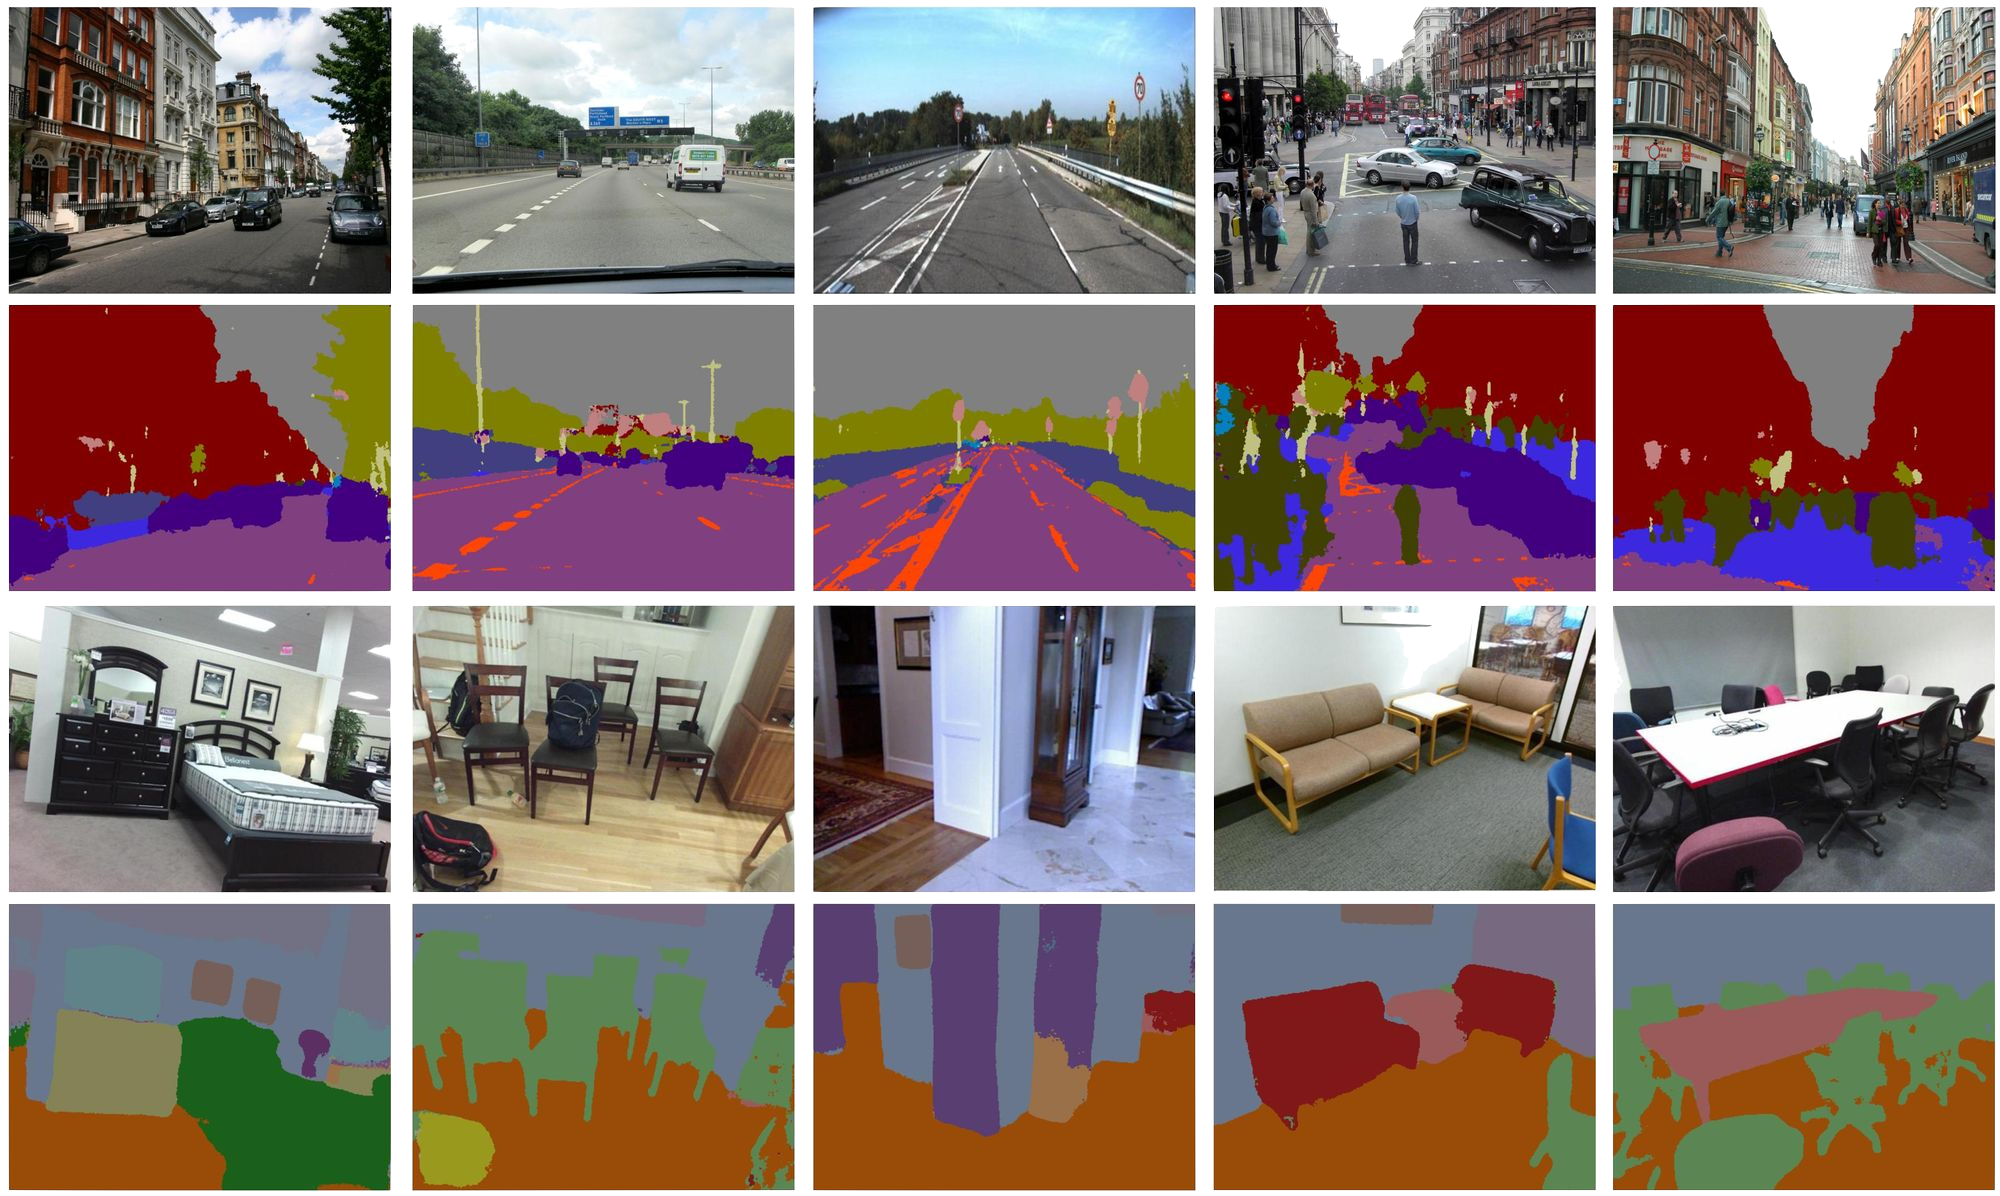
\includegraphics[width=.8\textwidth]{segment.png}
	\end{center}
	First step in \emph{multi-objects classification} and \emph{scene understanding}. Harder than classifying single objects.
\end{frame}

\begin{frame}
	\frametitle{end-to-end image segmentation}
	\textbf{Model:} Input is image $\vec{x}$, output is image $\vec{m}$ that has the same size as $\vec{x}$, but each pixel value is a label for a segmented region.
	\begin{center}
		\includegraphics[width=.8\textwidth]{deepseg.png}
	\end{center}
	Now our training process is actually \emph{supervised}, but uses the same structure as an autoencoder.
\end{frame}

\begin{frame}
	\frametitle{end-to-end image coloration}
	\textbf{Model:} Input is black and white image $\vec{x}$, output is colorized image $\vec{m}$. 
	\begin{center}
		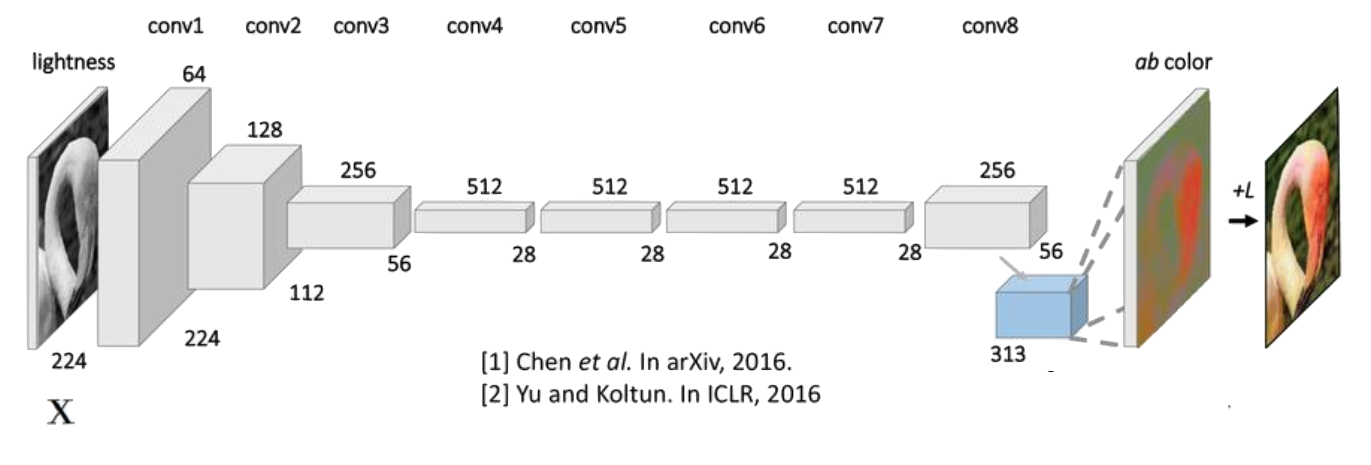
\includegraphics[width=.8\textwidth]{colorizer.png}
		
		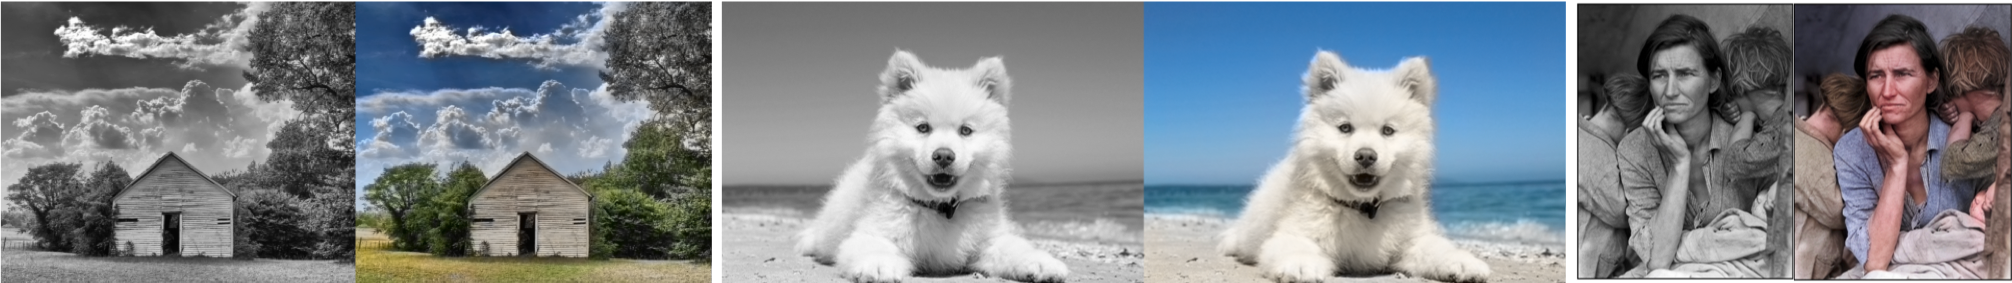
\includegraphics[width=\textwidth]{colorized_results.png}
	\end{center}
\end{frame}

\begin{frame}
	\frametitle{end-to-end super resolution}
	\textbf{Model:} Input is pixelated or blurred image $\vec{x}$, output is full-resolution image $\vec{m}$. 
	\begin{center}
		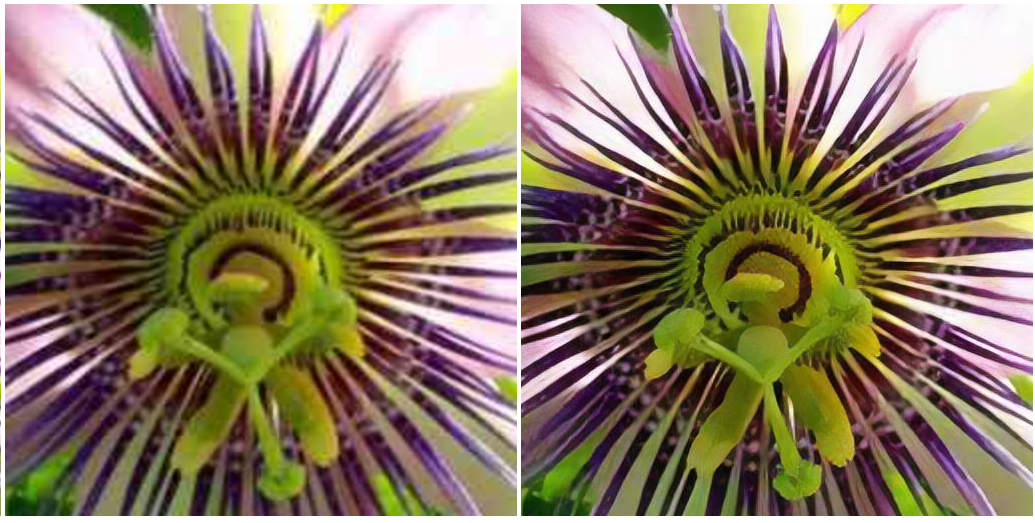
\includegraphics[width=.6\textwidth]{superresolution.png}
		
		 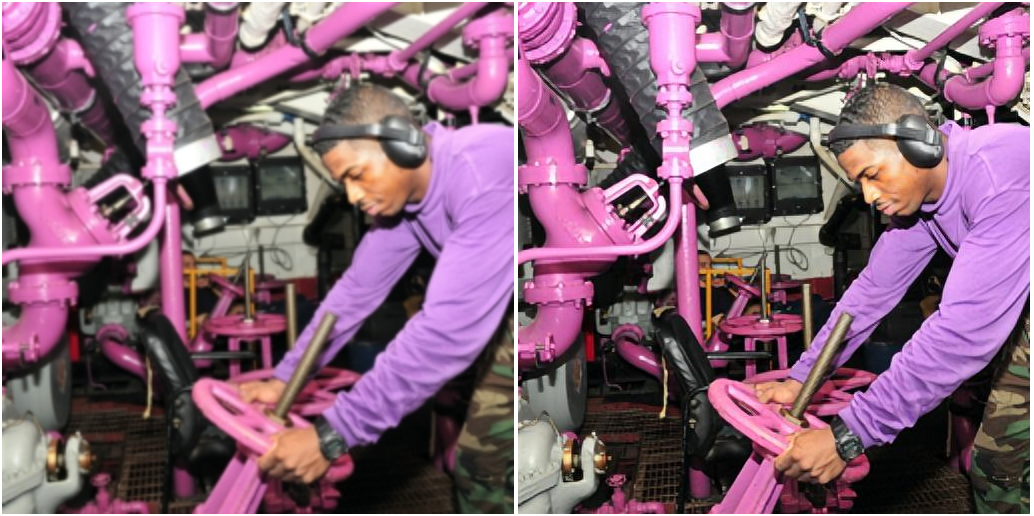
\includegraphics[width=.6\textwidth]{superresolution2.png}
	\end{center}
\end{frame}

\begin{frame}
	\frametitle{principal component analysis}
	\textbf{Simple \emph{linear} autoencoder:} Given input $\vec{x}\in \R^d$, 
		\begin{center}
		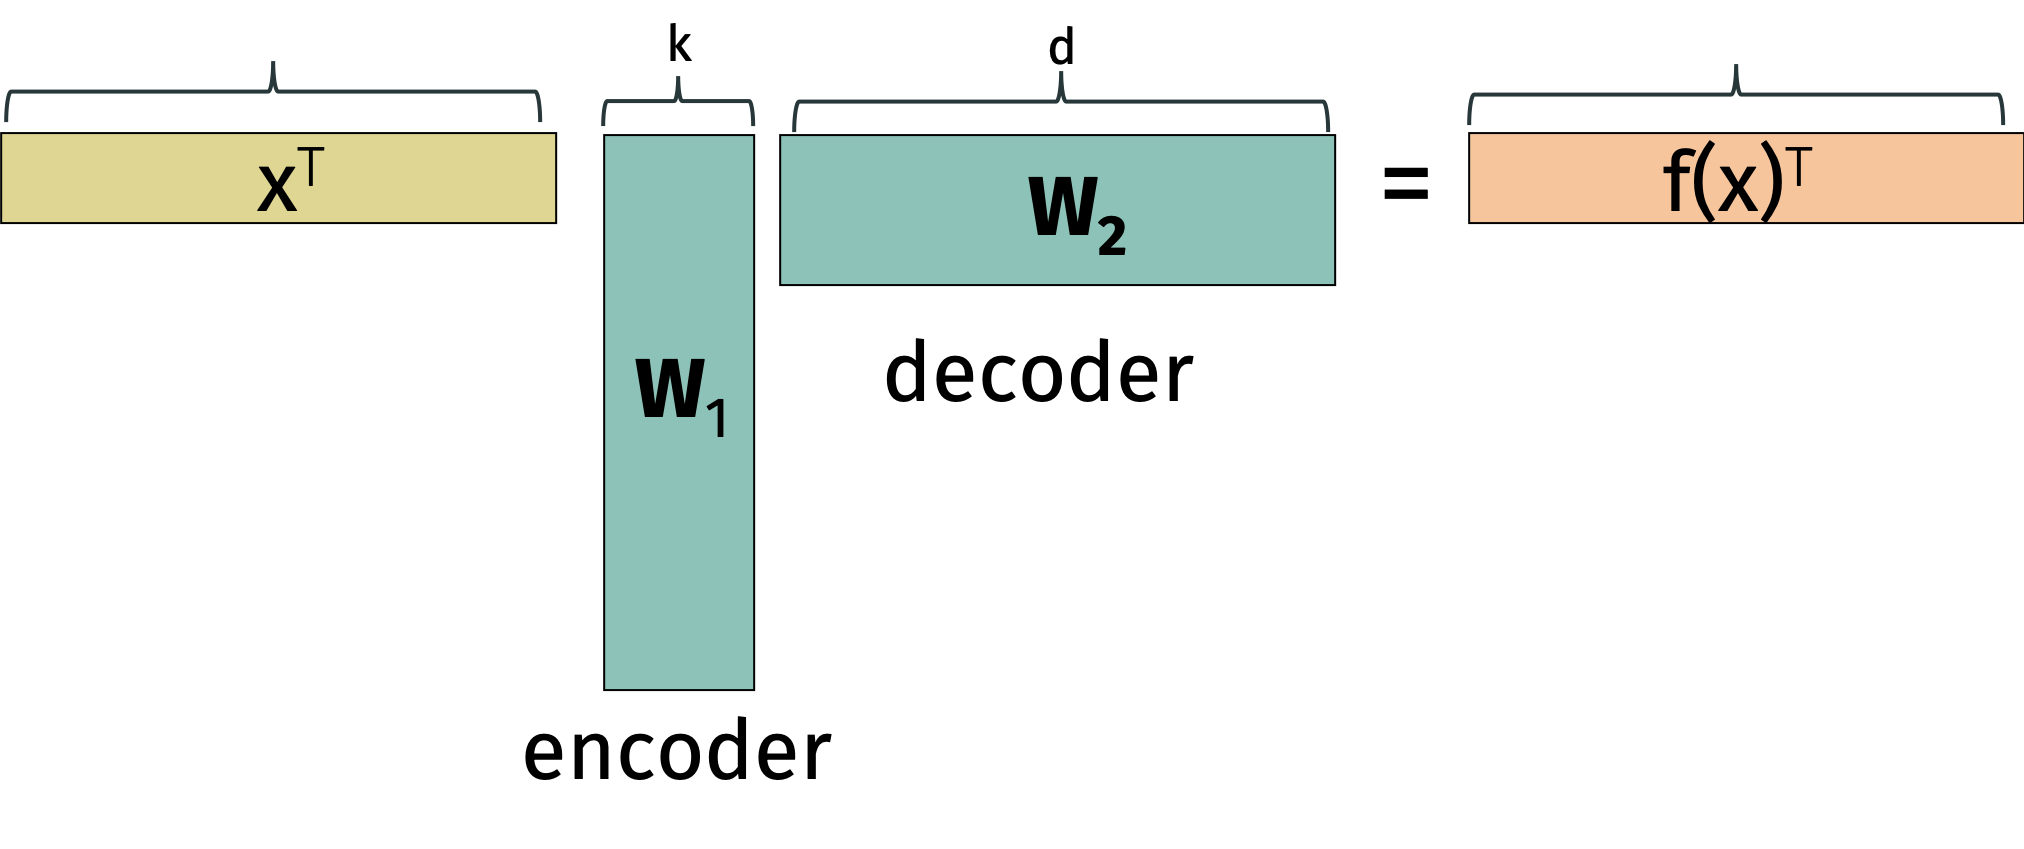
\includegraphics[width=.8\textwidth]{auto_alg.png}
	\end{center}
\begin{align*}
	f(\vec{x})^T = \vec{x}^T\bv{W}_1\bv{W}_2
\end{align*}
\end{frame}
\begin{frame}
	\frametitle{principal component analysis}
	\begin{center}
		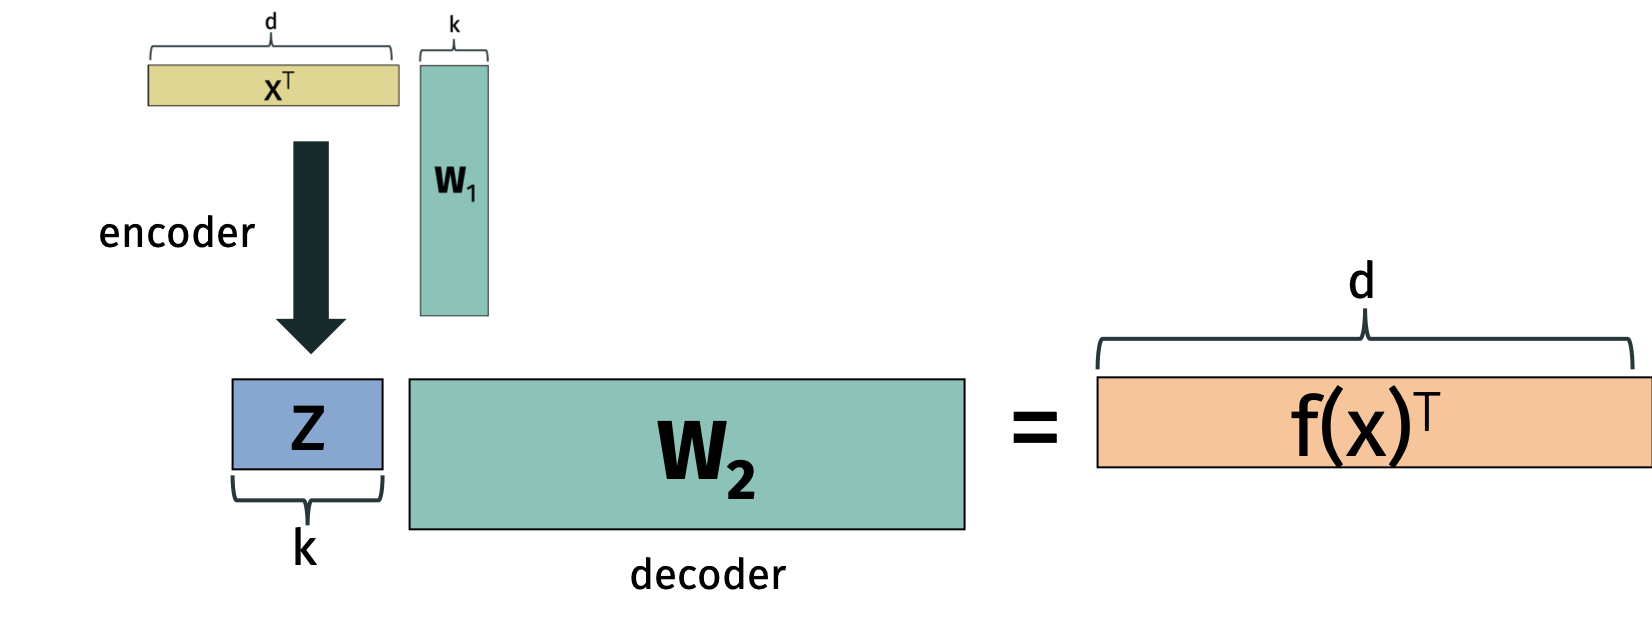
\includegraphics[width=.8\textwidth]{enc_dec.png}
	\end{center}
	\begin{center}
		\textbf{Encoder:} $e(\vec{x}) = \vec{x}^T \bv{W}_1$. \hspace{2em} \textbf{Decoder:} $d(\vec{z}) = \vec{z}\bv{W}_2$
	\end{center}
\end{frame}

\begin{frame}
	\frametitle{principal component analysis}
	Given training data set $\vec{x}_1, \ldots, \vec{x}_n$, let $\bv{X}$ denote our data matrix. Let  $\tilde{\bv{X}} = \bv{X}\bv{W}_1\bv{W}_2$.
	\begin{center}
		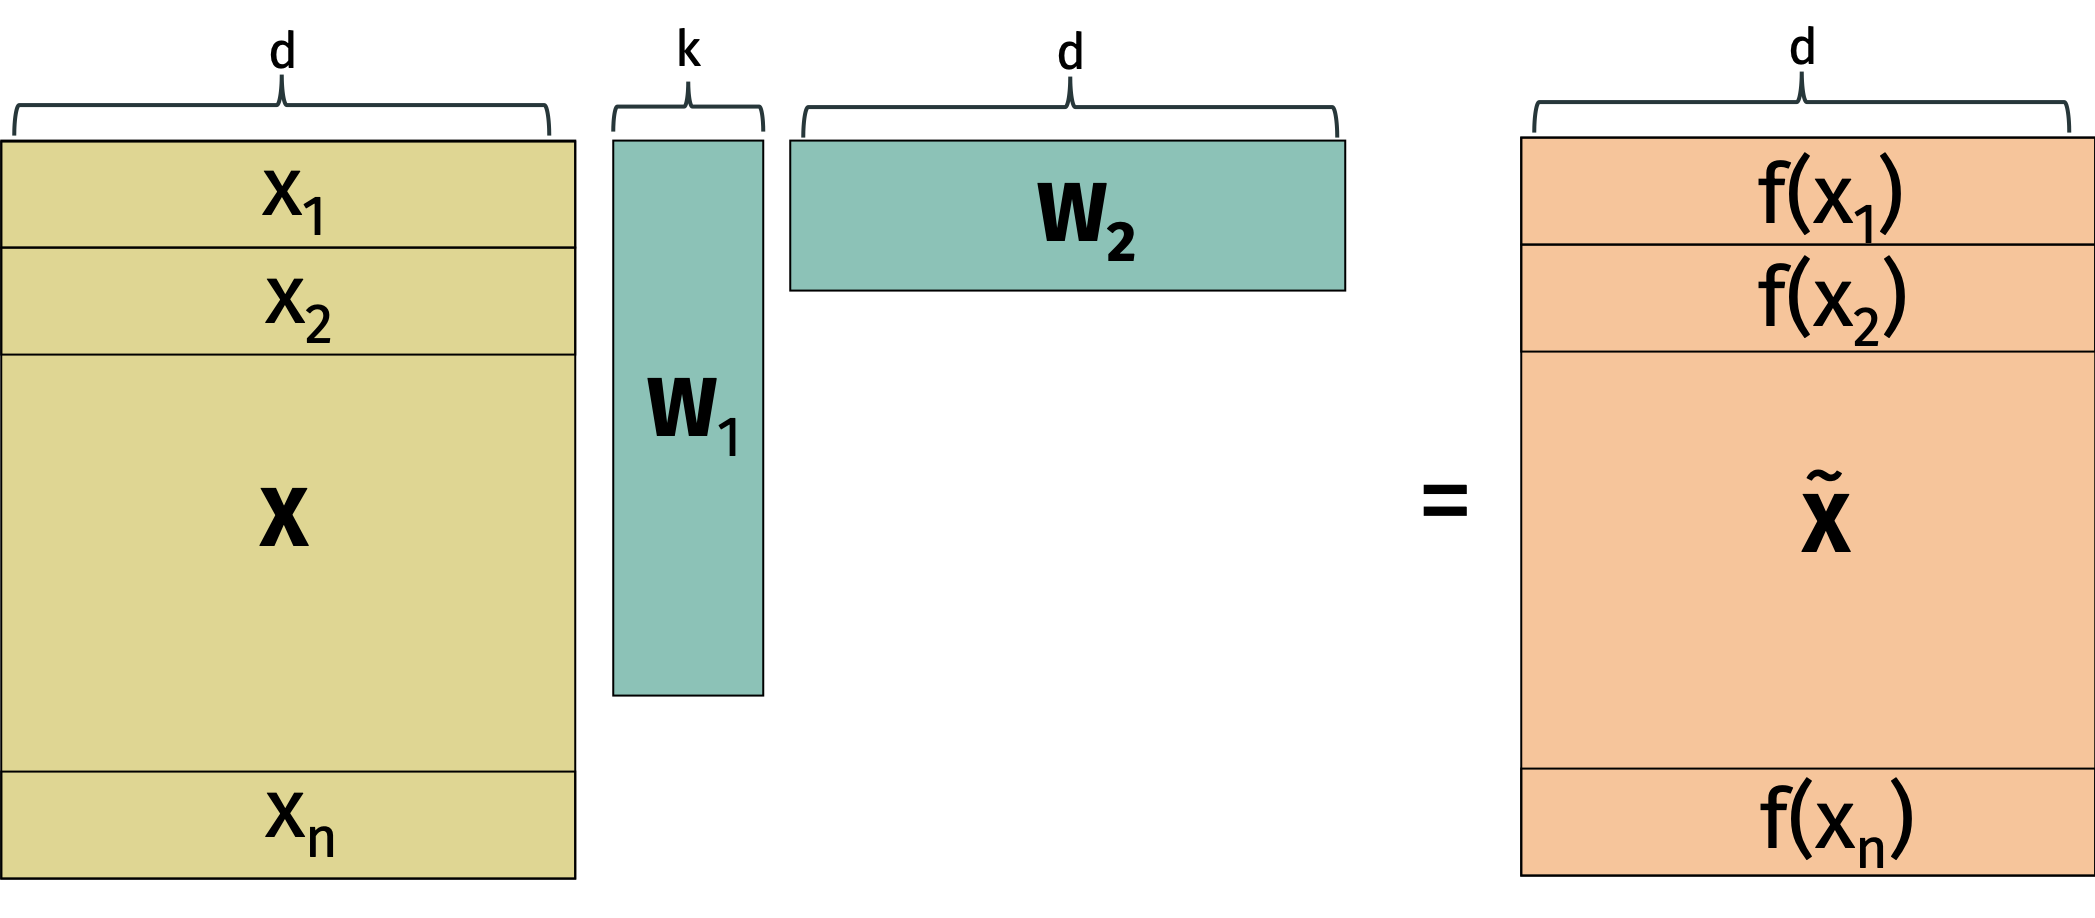
\includegraphics[width=.8\textwidth]{auto_alg_agg.png}
	\end{center}
	\textbf{Goal:} Find $\bv{W}_1, \bv{W}_2$ to minimize the Frobenius norm loss $\|\bv{X} - \tilde{\bv{X}}\|_F^2 = \|\bv{X} - \bv{X}\bv{W}_1\bv{W}_2\|_F^2$. 
\end{frame}

\begin{frame}
	\frametitle{low-rank approximation}
	\small
	\textbf{Recall:} \vspace{-.5em}
	
	\begin{itemize}
		\item The columns of a matrix with \emph{column rank} $k$ can all be written as linear combinations of just $k$ columns.\vspace{-.25em}
		\item The rows of a matrix with \emph{row rank} $k$ can all be written as linear combinations of $k$ rows.\vspace{-.25em}
		\item  Column rank = row rank = \textbf{rank}.\vspace{-.25em}
	\end{itemize} 
\vspace{-1em}
	\begin{center}
		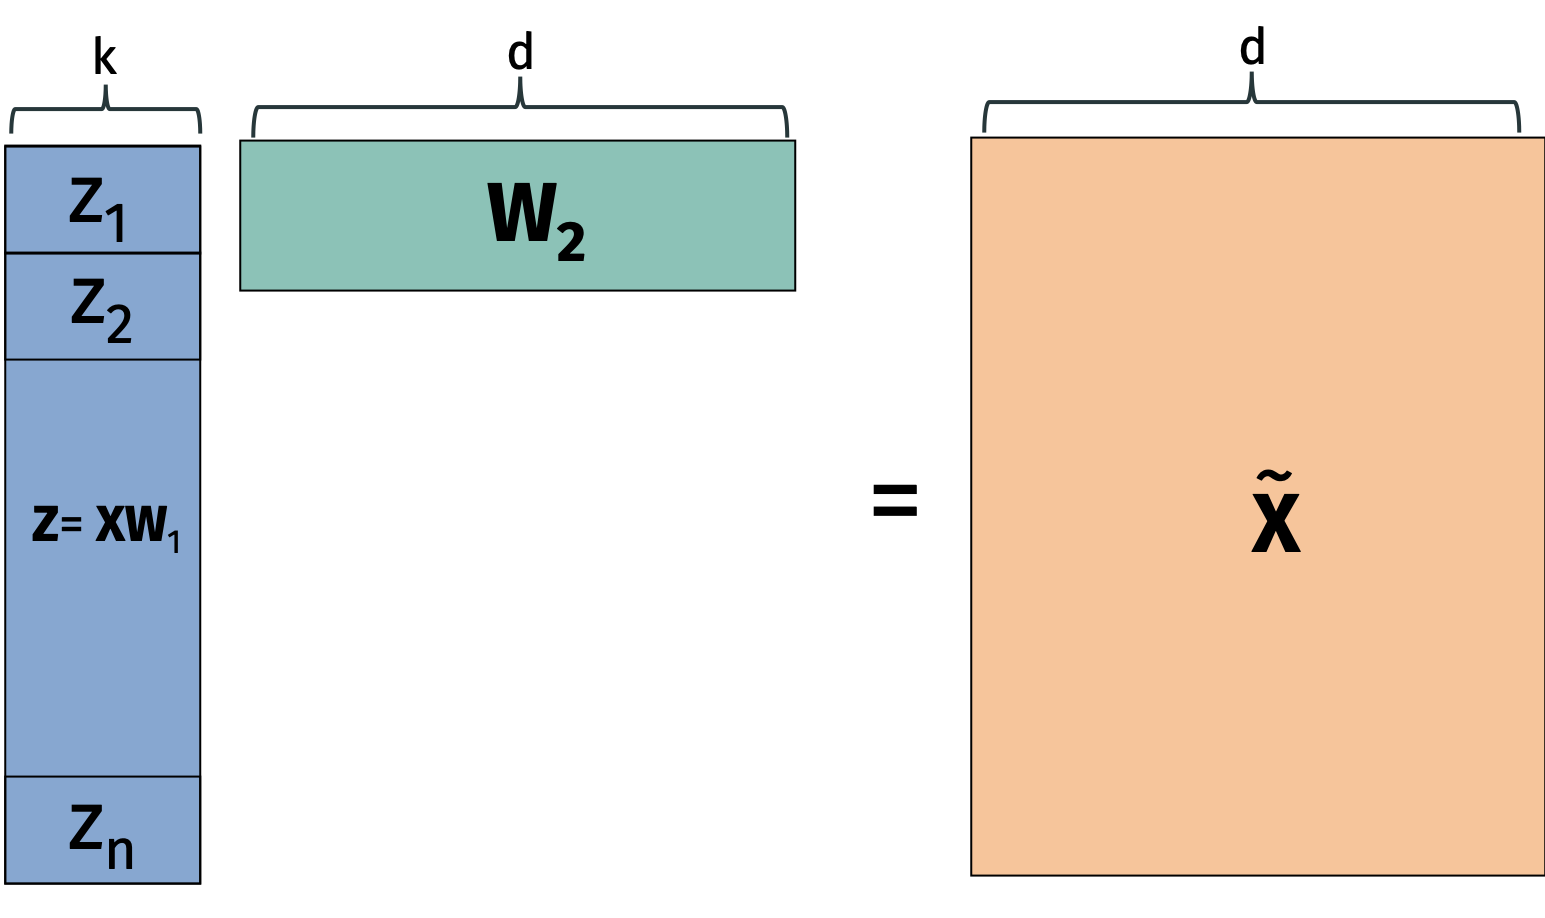
\includegraphics[width=.6\textwidth]{lowranktilde.png}
		
		$\tilde{\bv{X}}$ is a \alert{\textbf{low-rank matrix}}. It only has rank $k$ for $k \ll d$.
	\end{center}
\end{frame}

\begin{frame}
	\frametitle{low-rank approximation}
	\textbf{Principal component analysis} amounts to finding a rank $k$ matrix $\tilde{\bv{X}}$ which approximates the data matrix $\bv{X}$ as closely as possible. 
	
	In general, $\bv{X}$ will have rank $d$. 
\end{frame}

\begin{frame}
	\frametitle{singular value decomposition}
	\small
	\emph{Any} matrix $\bv{X}$ can be written:
	\begin{center}
		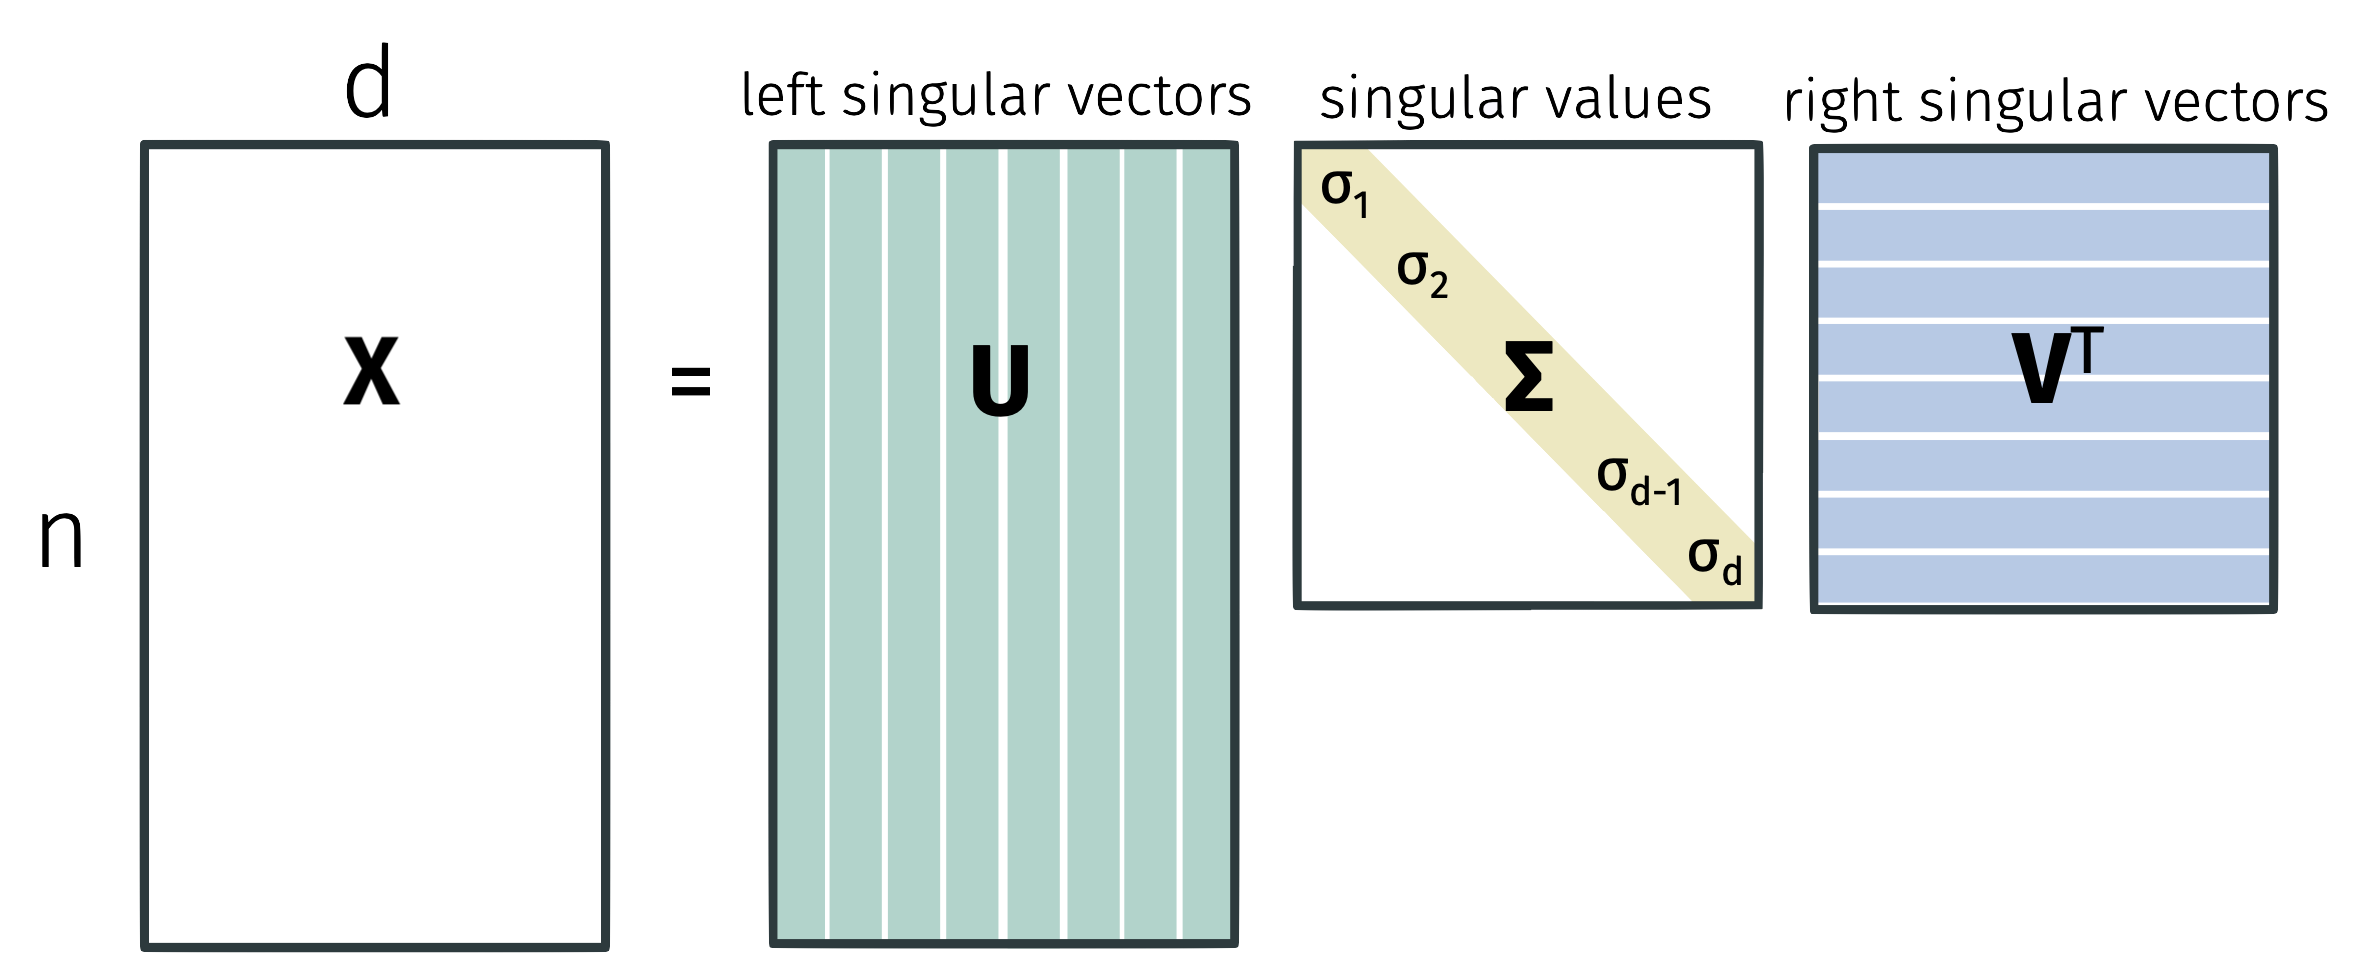
\includegraphics[width=.9\textwidth]{svd.png}
	\end{center} 
	Where $\bv{U}^T\bv{U} = \bv{I}$,  $\bv{V}^T\bv{V} = \bv{I}$, and $\sigma_1 \geq \sigma_2 \geq \ldots \sigma_d \geq 0$. I.e. $\bv{U}$ and $\bv{V}$ are \emph{orthogonal matrices}.
	\begin{center}
		\normalsize This is called the \textbf{singular value decomposition.}
	\end{center}
Can be computed in $O(nd^2)$ time (faster with approximation algos).
\end{frame}

\begin{frame}
	\frametitle{orthogonal matrices}
	Let $\bv{u}_1, \ldots, \bv{u}_n \in \R^n$ denote the columns of $\bv{U}$. I.e. the left singular vectors of $\bv{X}$. 
		\begin{center}
		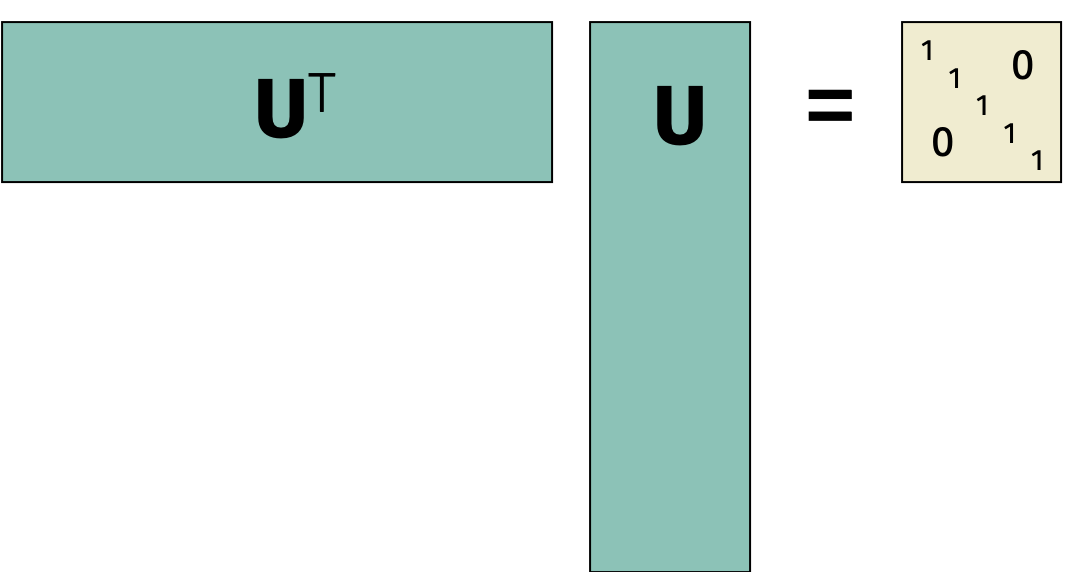
\includegraphics[width=.5\textwidth]{orthogonal.png}
	\end{center}
\begin{center}
	$\|u_i\|_2^2 = $ \hspace{8em} $\bv{u}_i^T\bv{u}_j = $
\end{center}
	
\end{frame}

\begin{frame}[t]
	\frametitle{singular value decomposition}
	Can read off optimal low-rank approximations from the SVD:
	\begin{center}
		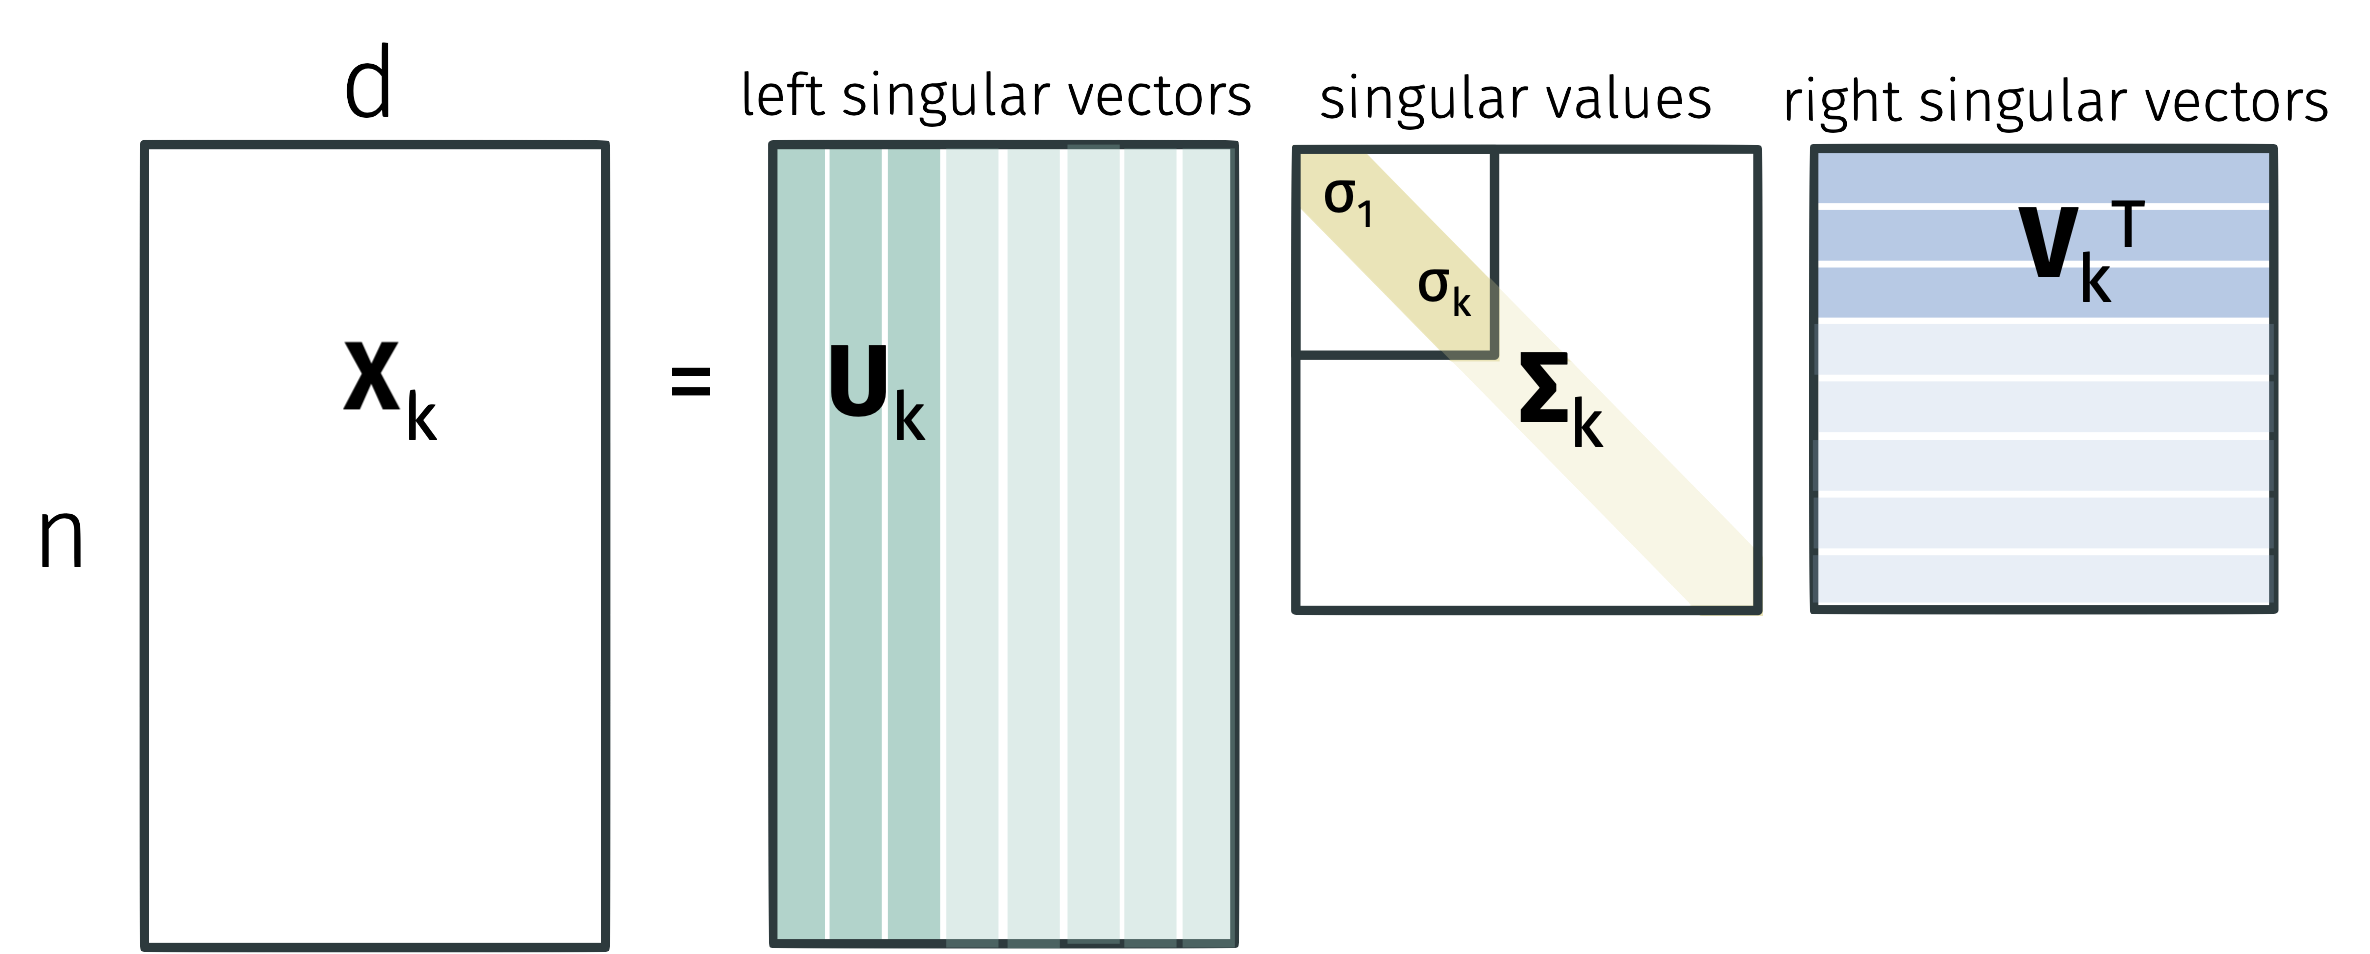
\includegraphics[width=.9\textwidth]{svdk.png}
	\end{center} 
	\textbf{Eckart–Young–Mirsky Theorem:} For any $k \leq d$, $\bv{X}_k = \bv{U}_k\bs{\Sigma}_k\bv{V}_k^T$ is the optimal $k$ rank approximation to $\bv{X}$:
	\begin{align*}
	\bv{X}_k = 	\argmin_{\tilde{\bv{X}} \text{ with rank $\leq k$} } \|\bv{X} - \tilde{\bv{X}}\|_F^2.
	\end{align*}
\end{frame}

\begin{frame}[t]
	\frametitle{singular value decomposition}
	\textbf{Claim:} $\bv{X}_k = \bv{U}_k\bs{\Sigma}_k\bv{V}_k^T = \bv{X}\bv{V}_k\bv{V}_k^T$.
	\vspace{15em}
	
	So for a model with $k$ hidden variables, we obtain an \emph{optimal autoencoder} by setting $\bv{W}_1 =\bv{V}_k$, $\bv{W}_2 = \bv{V}_k^T$. $f(\vec{x}) = \vec{x}\bv{V}_k\bv{V}_k^T$.
\end{frame}

\begin{frame}[t]
	\frametitle{singular value decomposition}
	\begin{center}
		\textbf{Computing the SVD.}
	\end{center} 
	\begin{itemize}
		\item Full SVD:\\
		\texttt{U,S,V = scipy.linalg.svd(X)}. 
		\begin{center}
		\alert{Runs in $O(nd^2)$ time.}
		\end{center}
		\item Just the top $k$ components: \\
		
		\texttt{U,S,V = scipy.sparse.linalg.svds(X, k).} 
		\begin{center}
			\alert{Runs in \emph{roughly} $O(ndk)$ time.}
		\end{center}
		
	\end{itemize}	
\end{frame}

\begin{frame}[t]
	\frametitle{principal component analysis}
	\begin{center}
		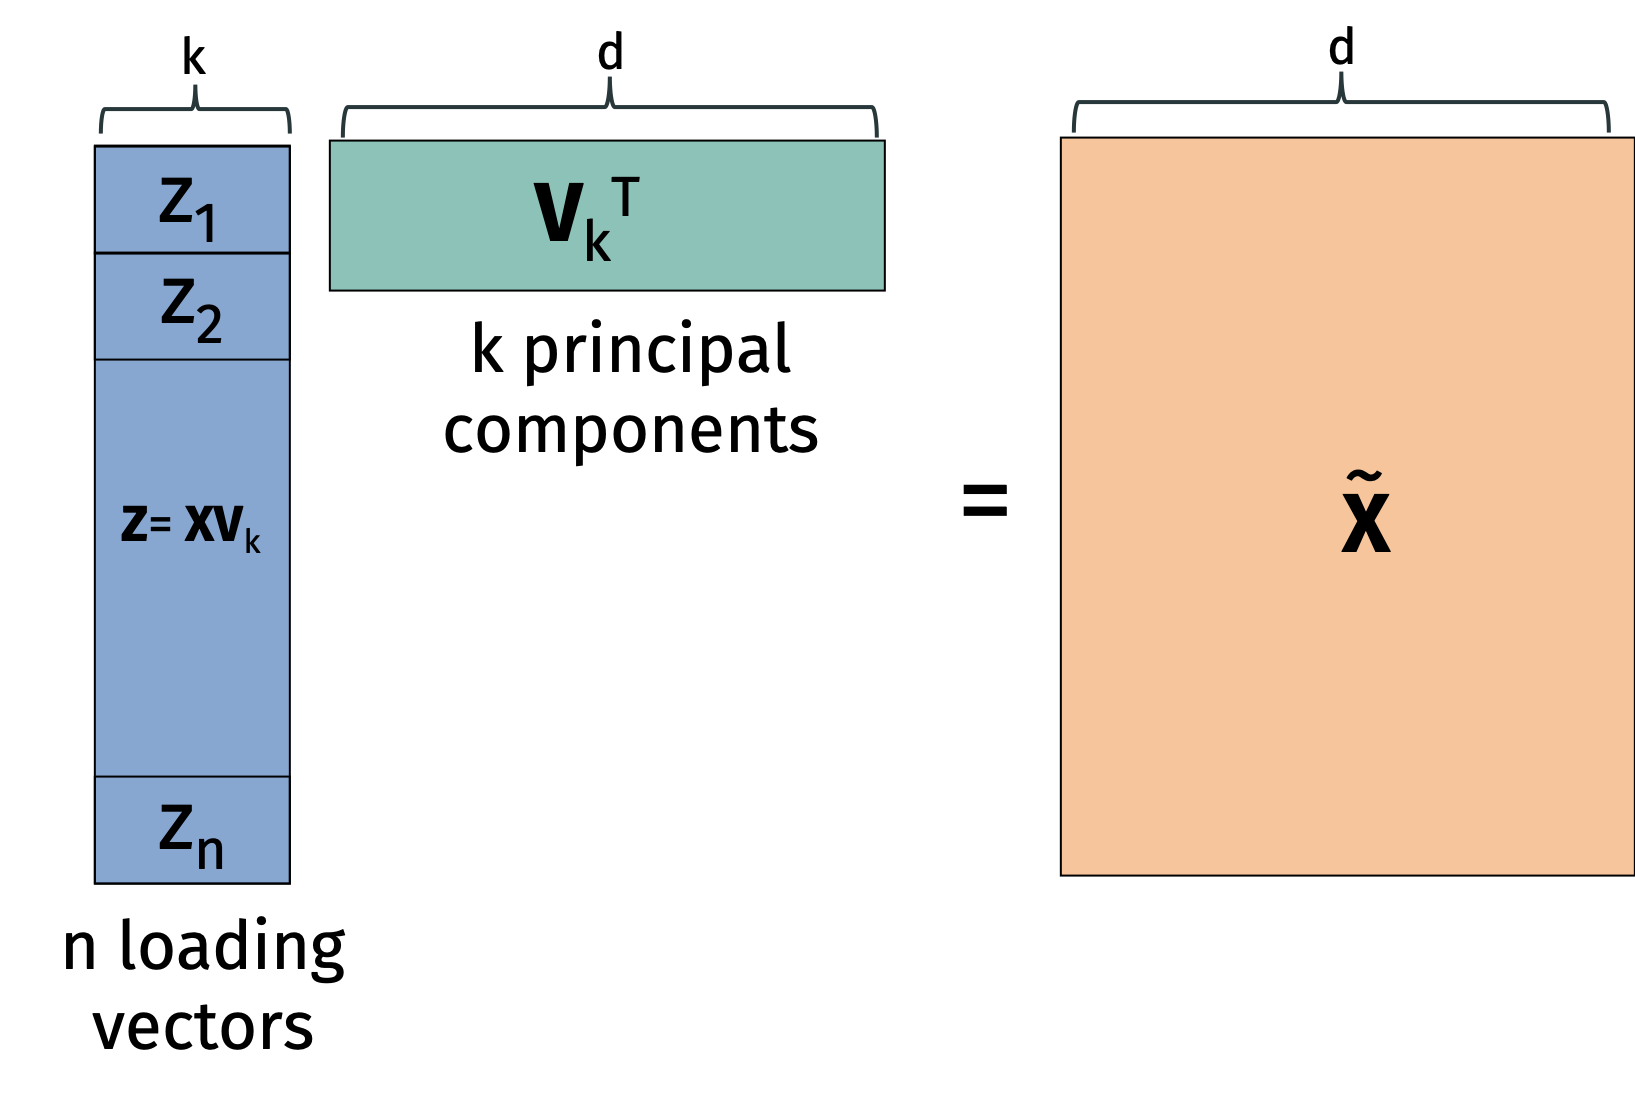
\includegraphics[width=.8\textwidth]{pca.png}
	\end{center} 
Usually $\vec{X}$'s columns (features) are mean centered and normalized to variance $1$ before computing principal components.
\end{frame}

\begin{frame}[t]
	\frametitle{low rank approximation}
	\begin{center}
	\vspace{-.5em}
	What does recovered data $\tilde{\bv{X}} = \bv{X}_k$ look like?
	
	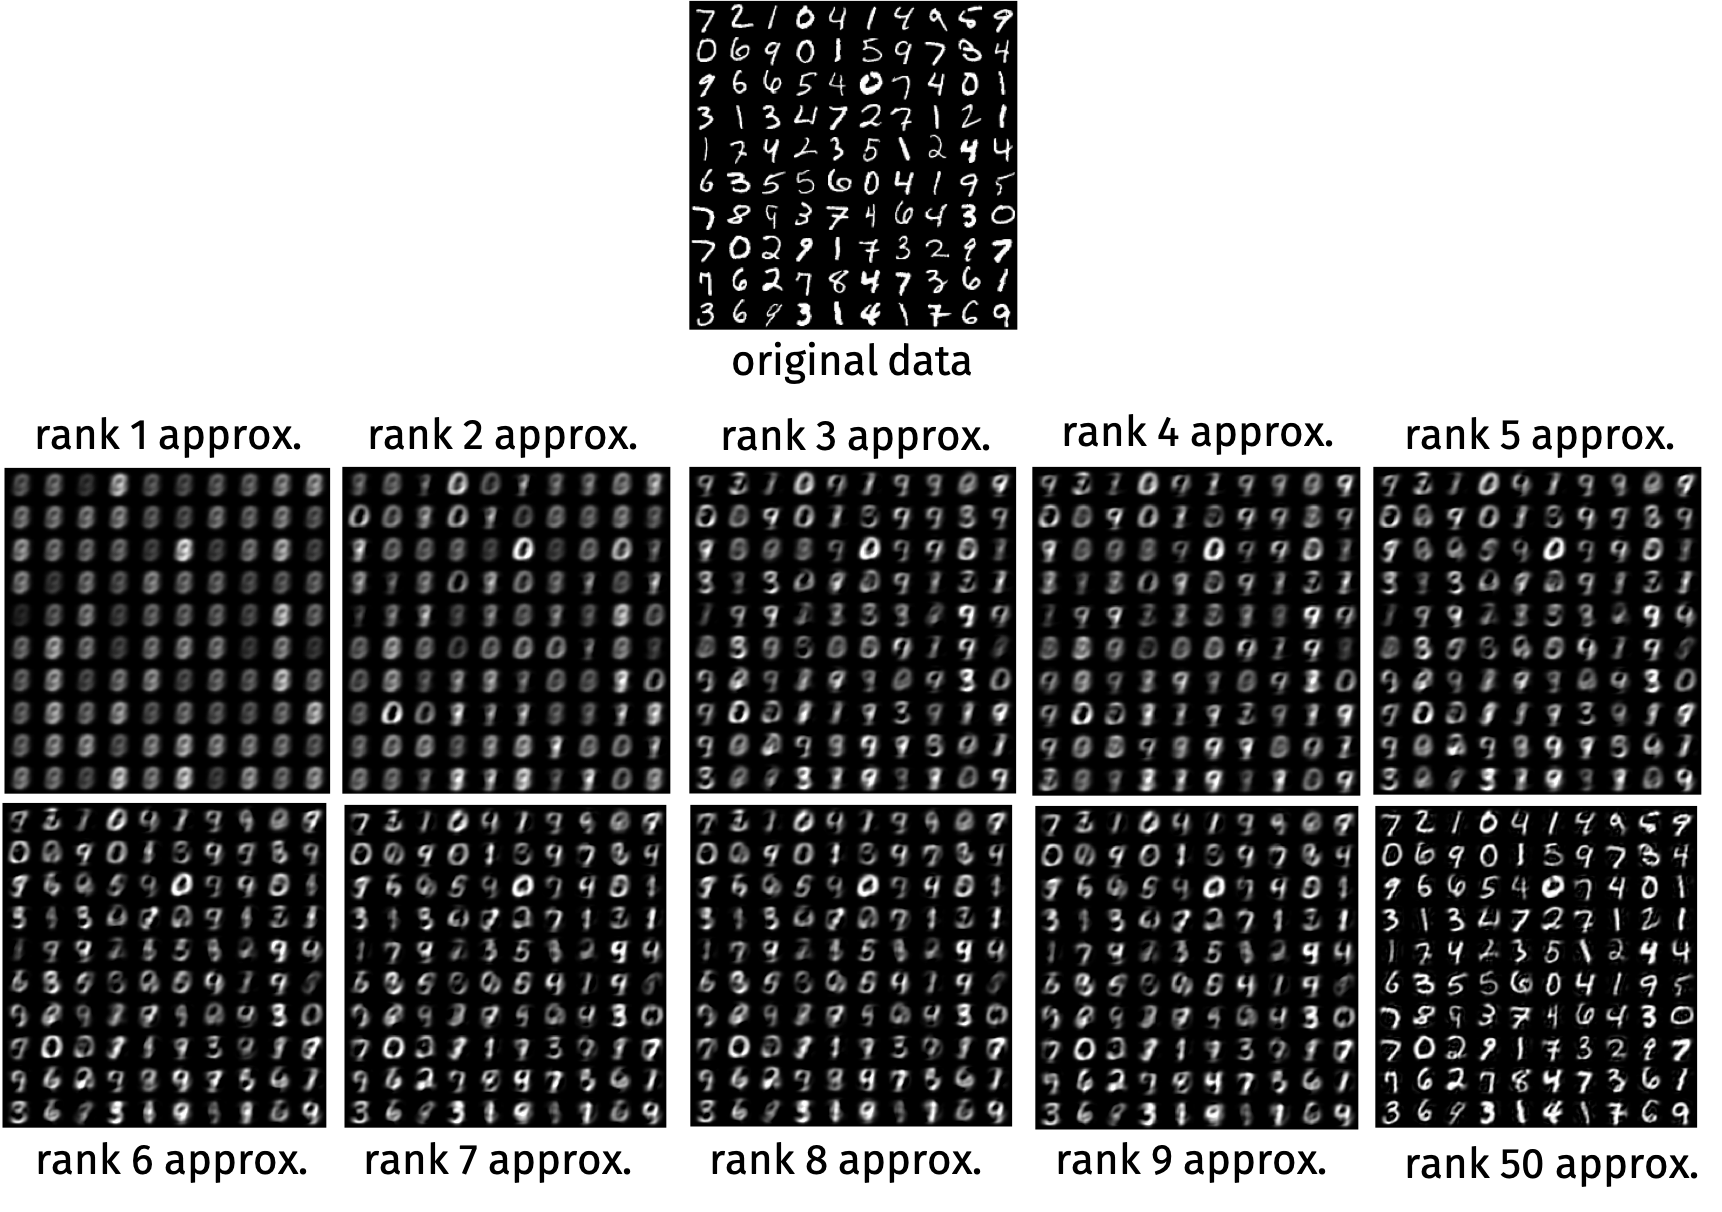
\includegraphics[width=.95\textwidth]{low_rank_approxs2.png}
	\end{center}
\end{frame} 

\begin{frame}[t]
	\frametitle{low rank approximation}
	The error can be written as:
	\begin{align*}
	\|\bv{X} - \bv{X}_k\|_F^2 = \sum_{i=k}^d \sigma_i^2.
	\end{align*} 
	\begin{center}
		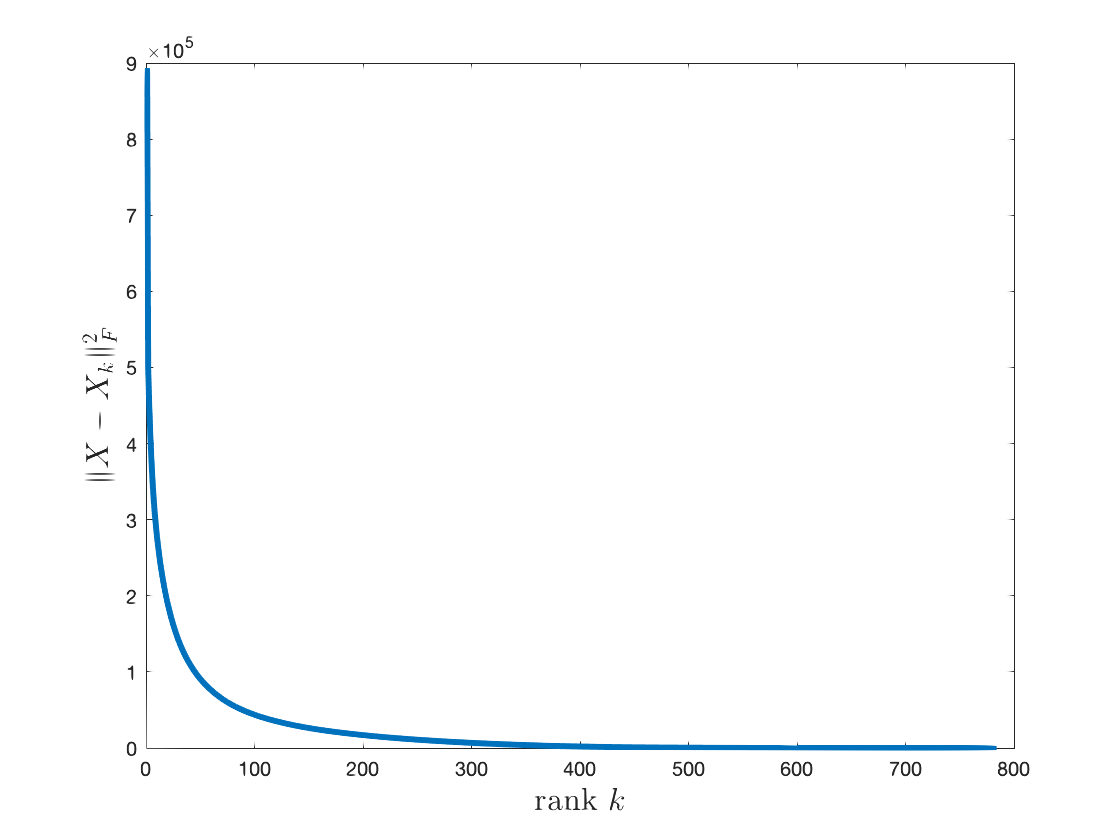
\includegraphics[width=.6\textwidth]{pca_errors.png}
	\end{center}
	
\end{frame}


\begin{frame}[t]
	\frametitle{principal components}
	What do the \textbf{principal components} looks like? 
	
	Want a small set of vector $\vec{v}_1, \ldots, \vec{v}_k$ so that most data examples $\vec{x}$ can be written as a linear combination of these \emph{basis} vectors:
	\begin{align*}
	\vec{x}\approx c_1 \vec{v}_1 + c_2 \vec{v}_2 + \ldots + c_k\vec{v}_k
	\end{align*}
	
	\textbf{One possible basis:} 
\includegraphics[width=.9\textwidth]{basis1.png}
	
	\textbf{More compact basis:} 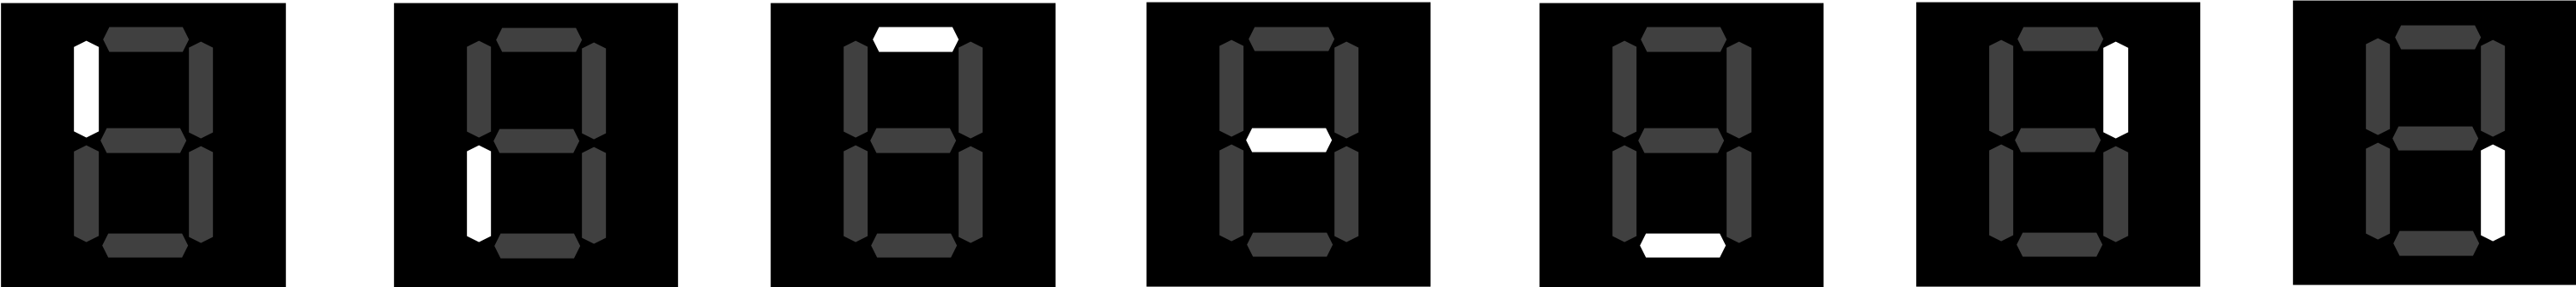
\includegraphics[width=.7\textwidth]{digital3.png}
	
\end{frame}



\begin{frame}[t]
	\frametitle{principal components}
	\begin{center}
		\vspace{-.5em}
		MNIST \textbf{principal components}: 
		
		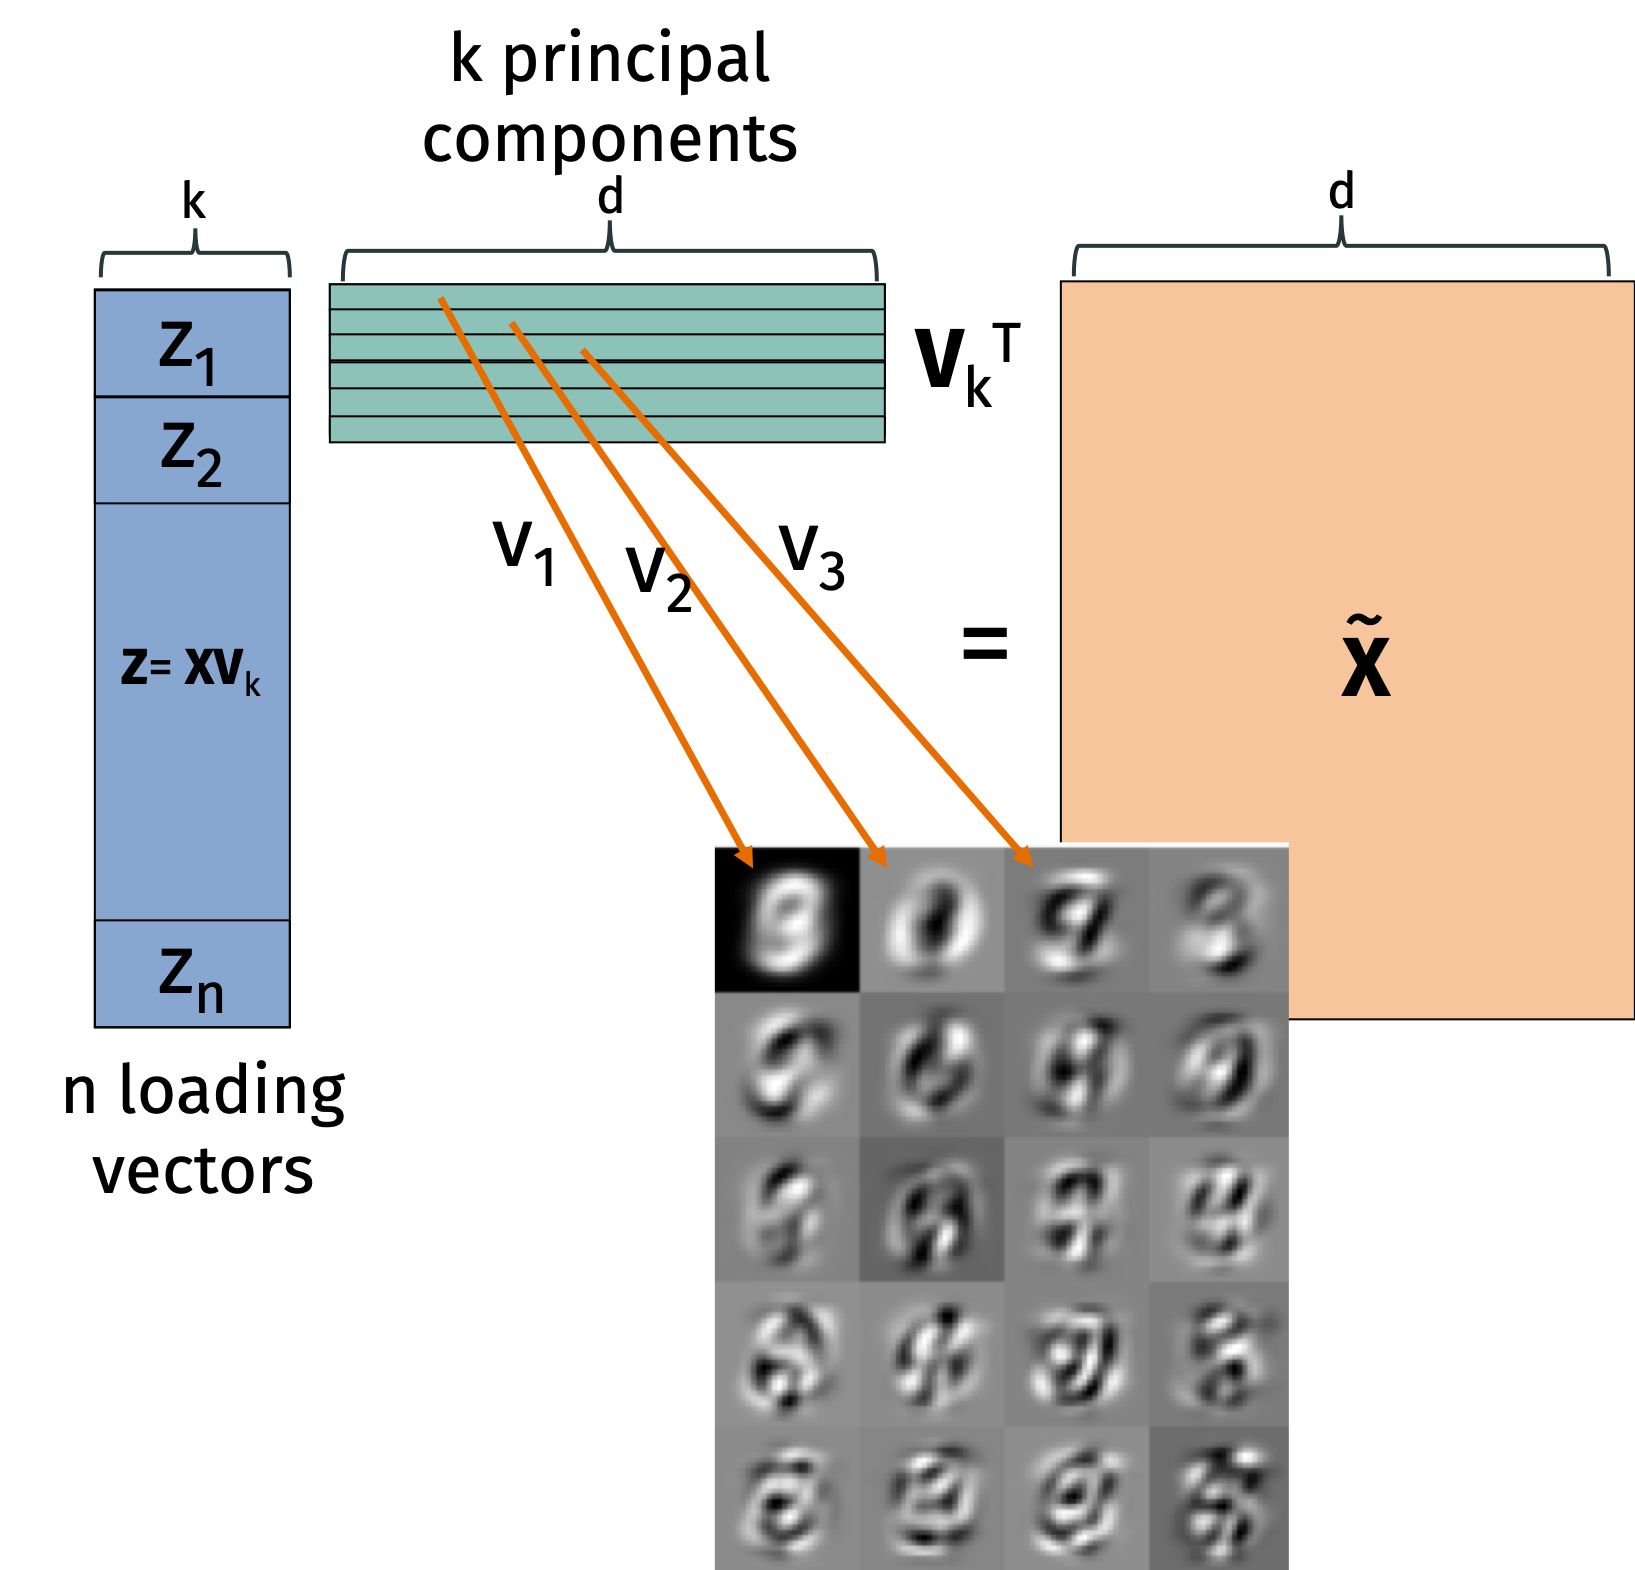
\includegraphics[width=.6\textwidth]{pc_visualization.png}
		
			Often principal components are difficult to interpret.
	\end{center}
\end{frame}

\begin{frame}[t]
	\frametitle{loading vectors}
	\small
	\begin{center}
			What do the \textbf{loading vectors} looks like? 
		
		The loading vector $\vec{z}$ for an example $\vec{x}$ contains coefficients which recombine the top $k$ principal components $\vec{v}_1, \ldots, \vec{v}_k$ to approximately reconstruct $\vec{x}$. 
		
		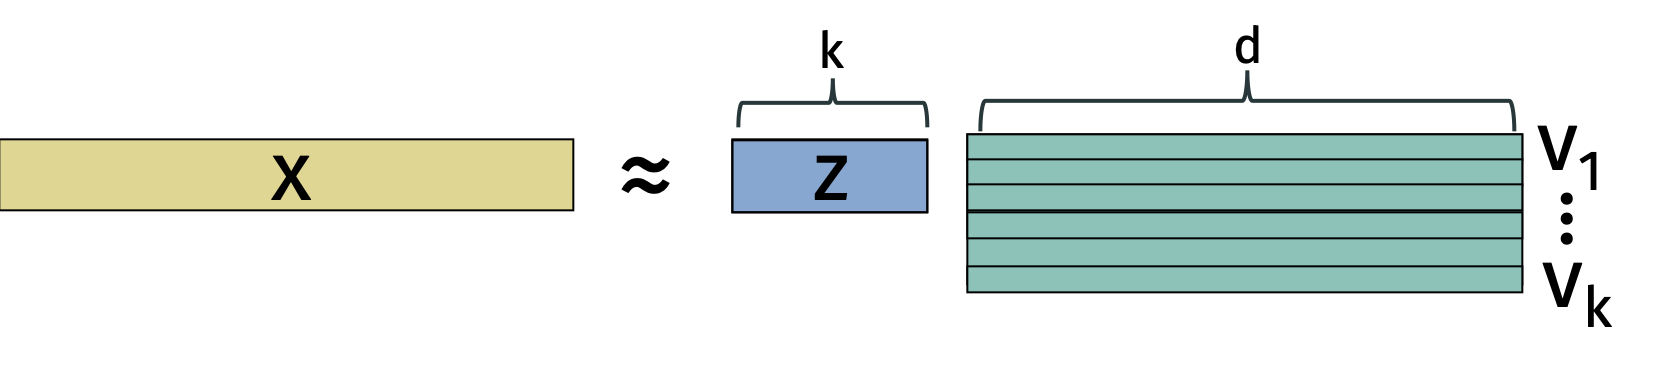
\includegraphics[width=.8\textwidth]{loading_diag.png}

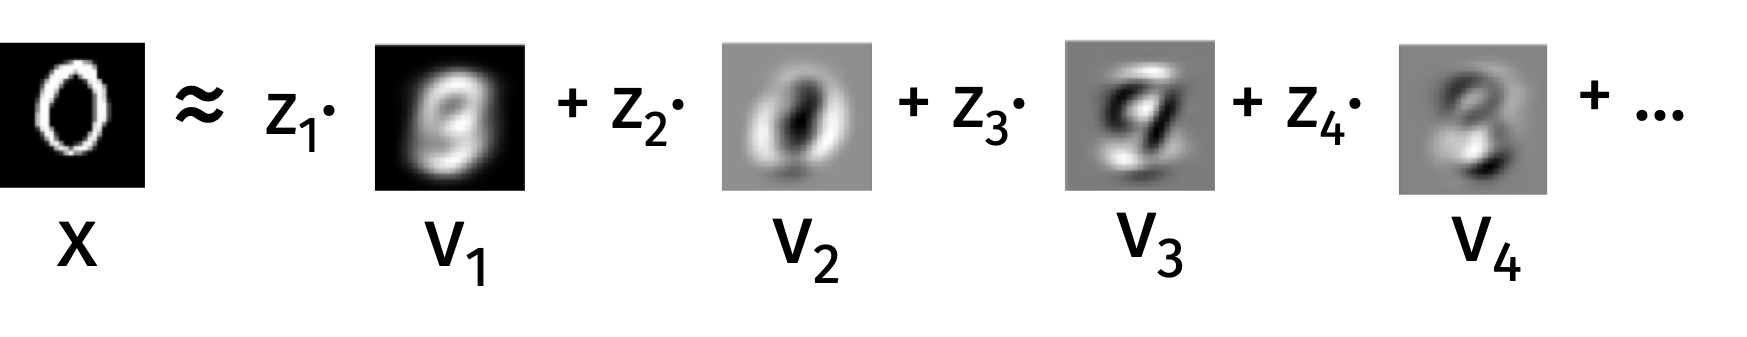
\includegraphics[width=.8\textwidth]{loadingexamp.png}

Provide a short ``finger print'' for any image $\vec{x}$ which can be used to reconstruct that image. 
	\end{center}
\end{frame}

\begin{frame}[t]
	\frametitle{loading vectors: similarity view}
	For any $\vec{x}$ with loading vector $\vec{z}$, $z_i$ is the inner product similarity between $\vec{x}$ and the $i^\text{th}$ principal component $\vec{v}_i$. 
	\begin{center}
		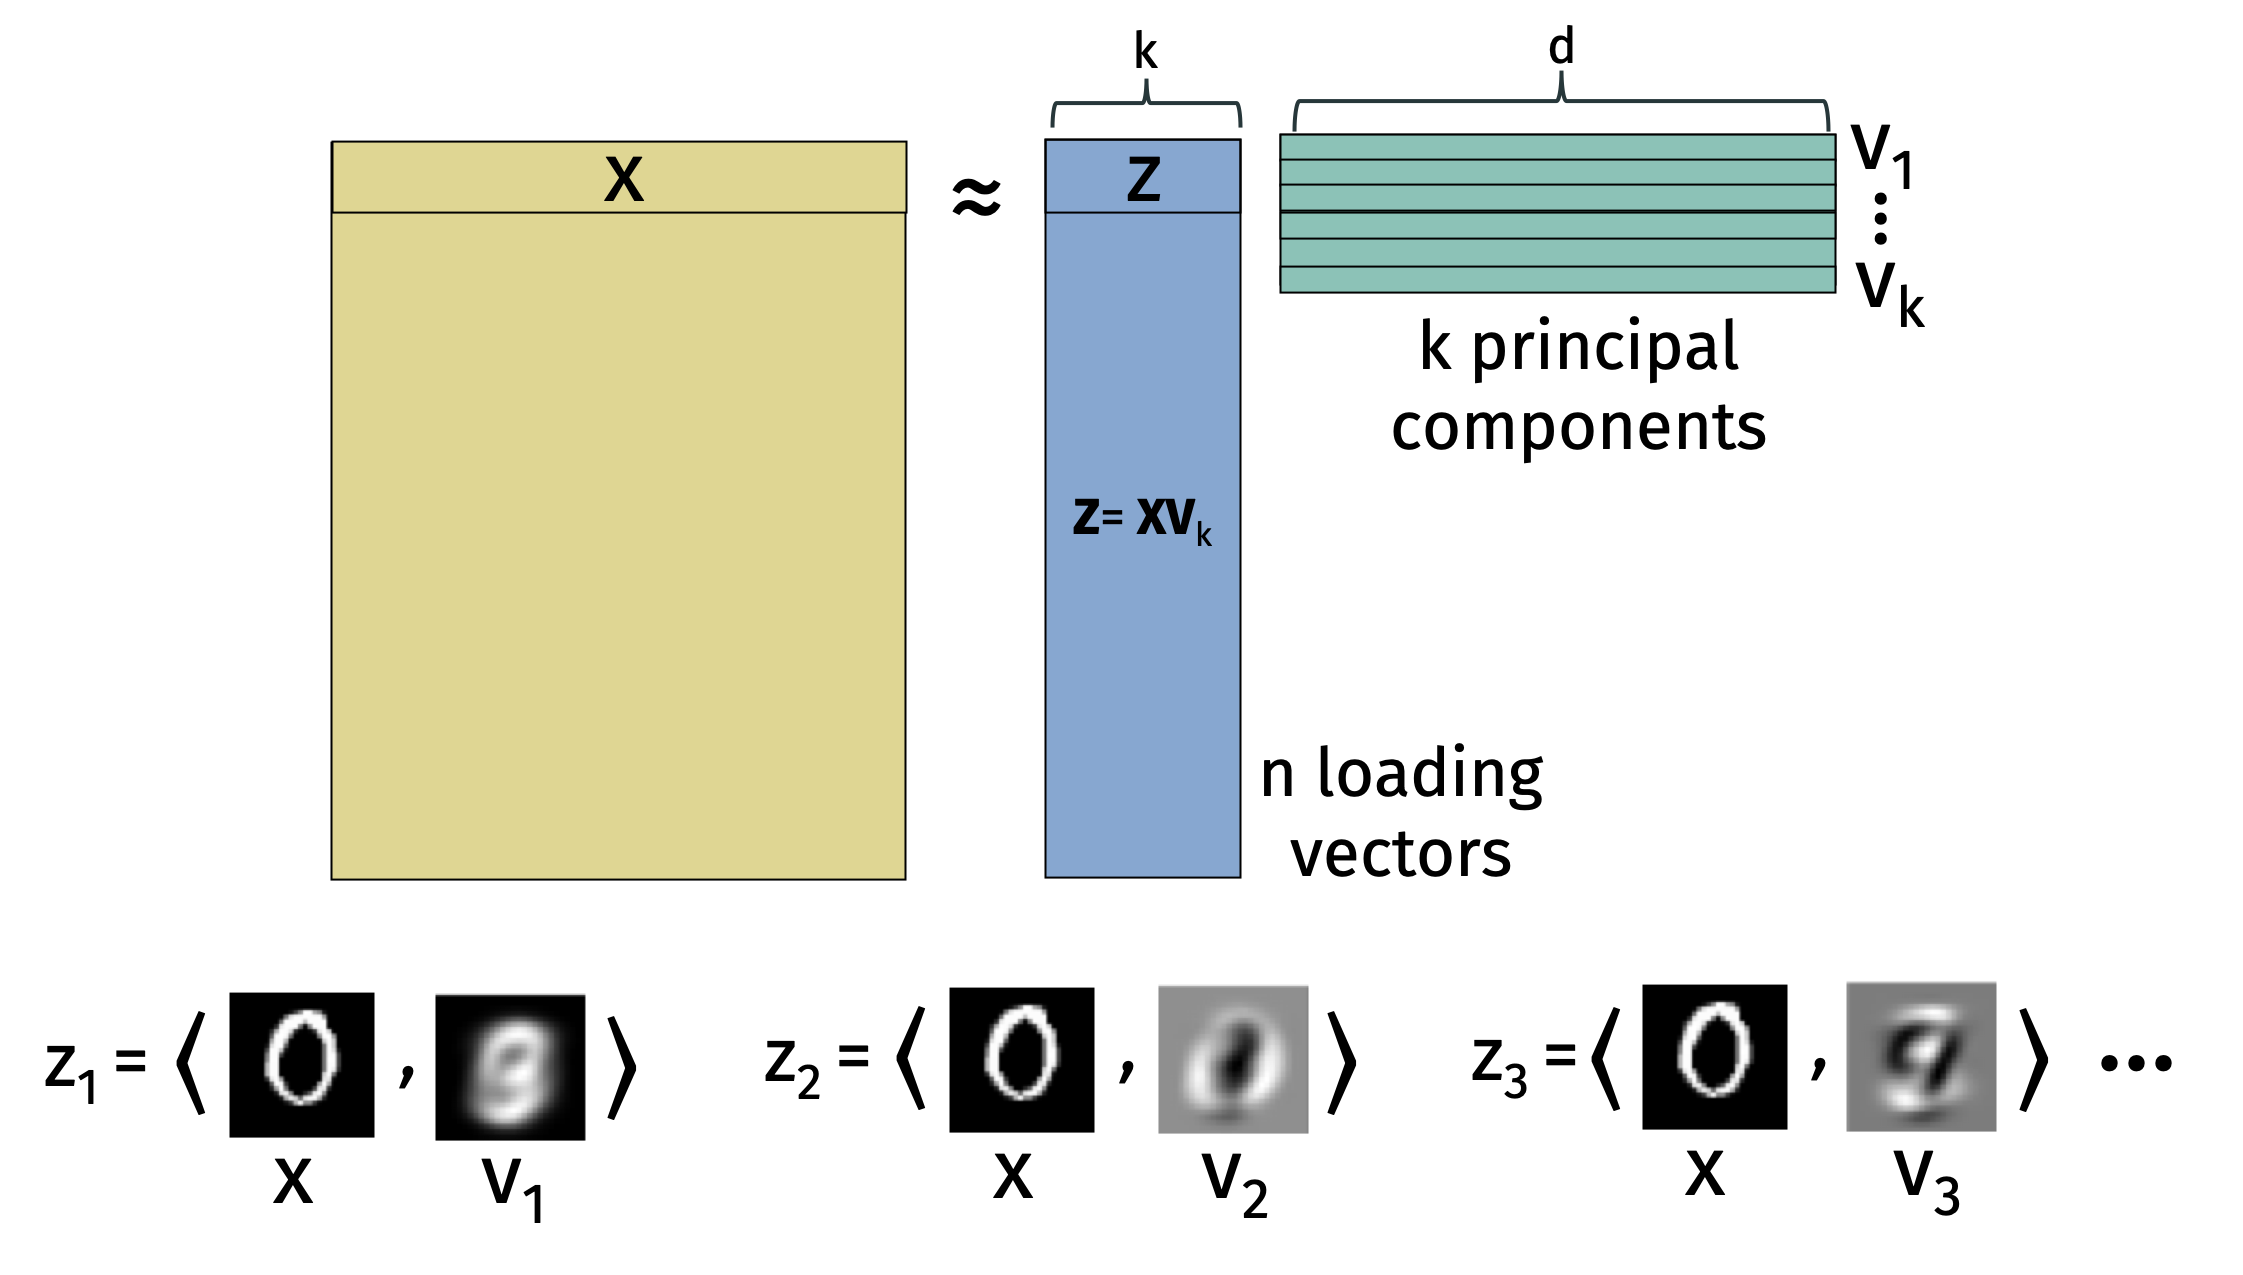
\includegraphics[width=.8\textwidth]{simview.png}
	\end{center}	
\end{frame}

\begin{frame}[t]
	\frametitle{loading vectors: projection view}
	So we approximate $\vec{x} \approx \tilde{x} = \langle \vec{x},\vec{v}_1\rangle \cdot v_1 + \ldots + \langle \vec{x},\vec{v}_k\rangle \cdot \vec{v}_k$. 
	\begin{center}
		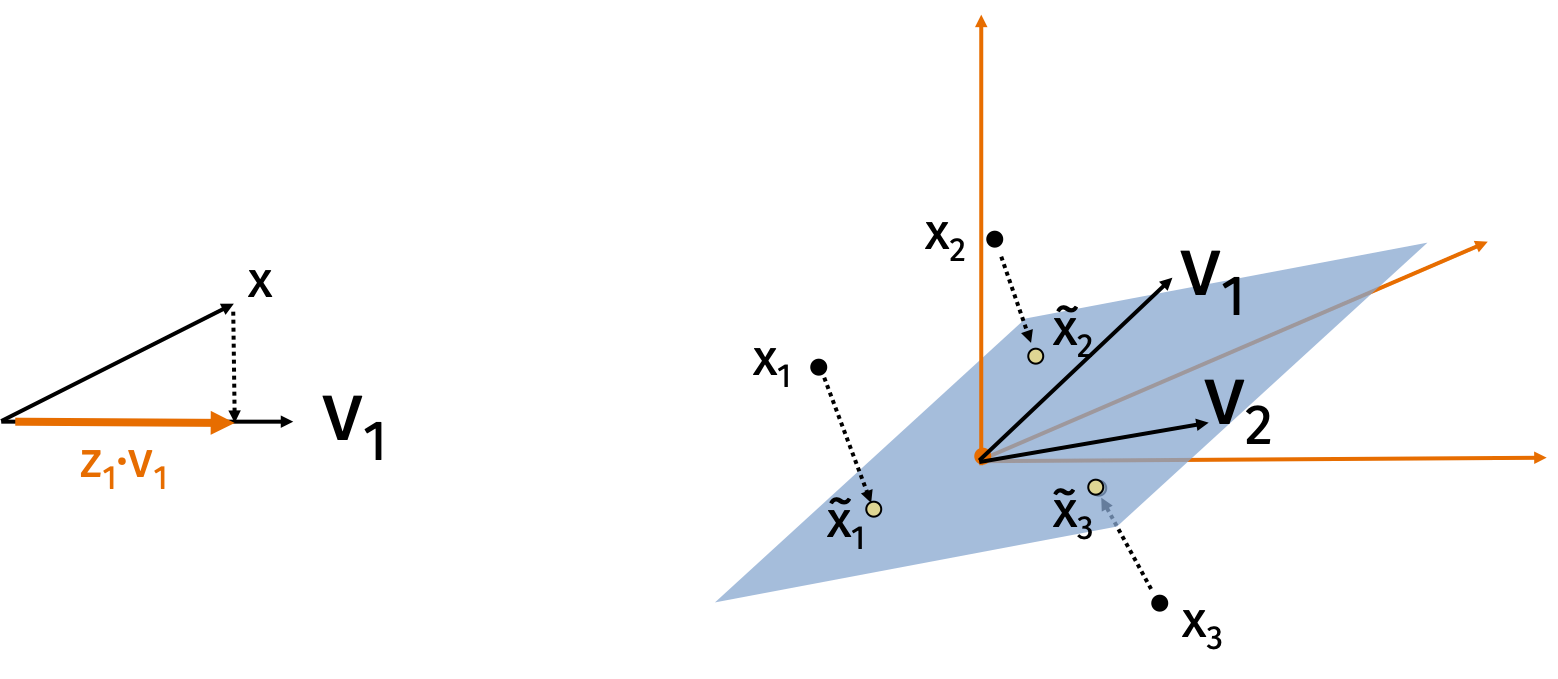
\includegraphics[width=.8\textwidth]{projection_orth.png}
		
		Projection onto first $2$ principal components.

	\end{center}
	Equivalent to projecting $\vec{x}$ onto the $k$-dimensional subspace spanned by $\vec{v}_1, \ldots, \vec{v}_k$. 
	
\end{frame}

\begin{frame}[t]
	\frametitle{loading vectors: projection view}
	For an example $\vec{x}_i$, the loading vector $\vec{z}_i$ contains the coordinates in the projection space:
	\begin{center}
		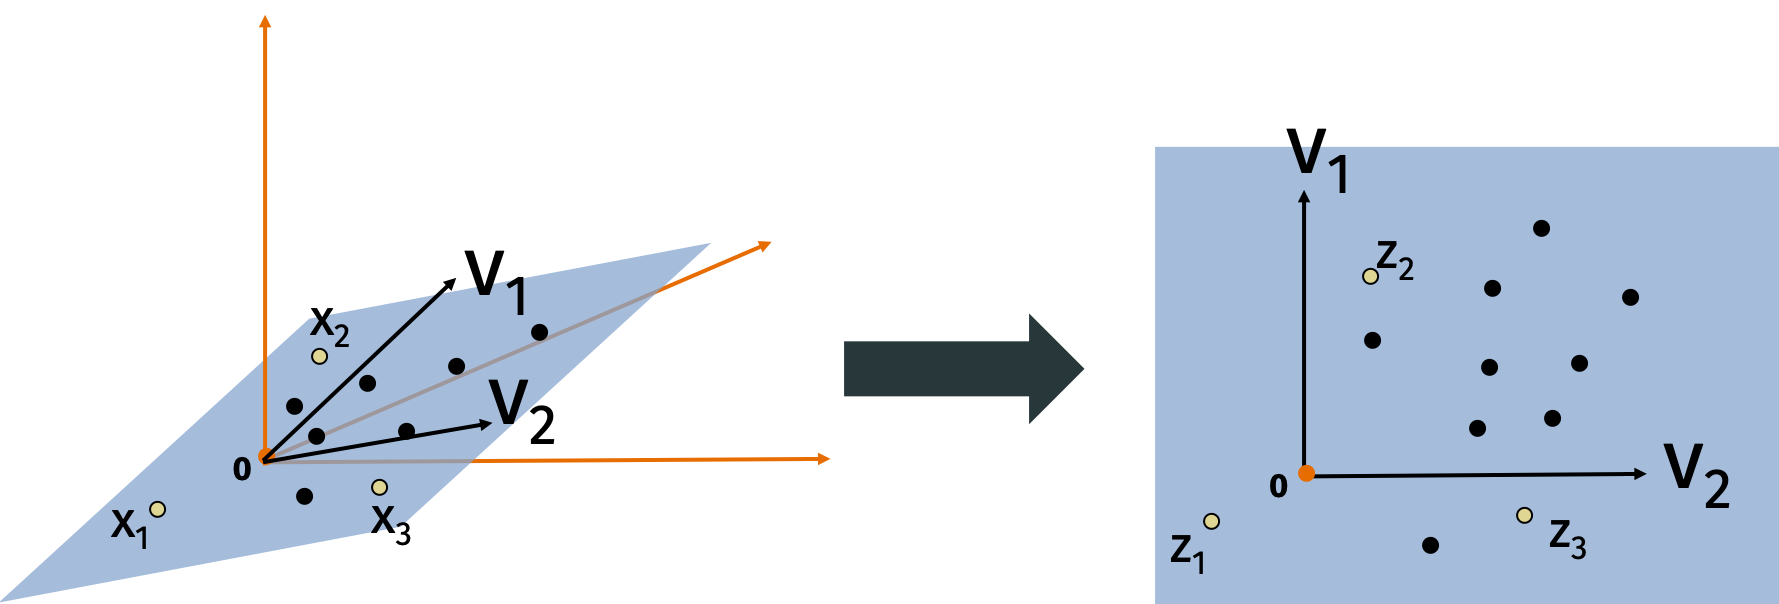
\includegraphics[width=\textwidth]{reparam.png}
		
		Projection onto first $2$ principal components.
		
	\end{center}
	
\end{frame}

\begin{frame}
	\frametitle{pca applications}
	\textbf{Like any autoencoder, PCA can be used for:}
	\begin{itemize}
		\item Feature extraction
		\item Denoising and rectification
		\item Data generation
		\item Compression
		\item Visualization
	\end{itemize}
\end{frame}

\begin{frame}
	\frametitle{pca for data visualization}
	``Genes Mirror Geography Within Europe'' -- Nature, 2008.
	\begin{center}
		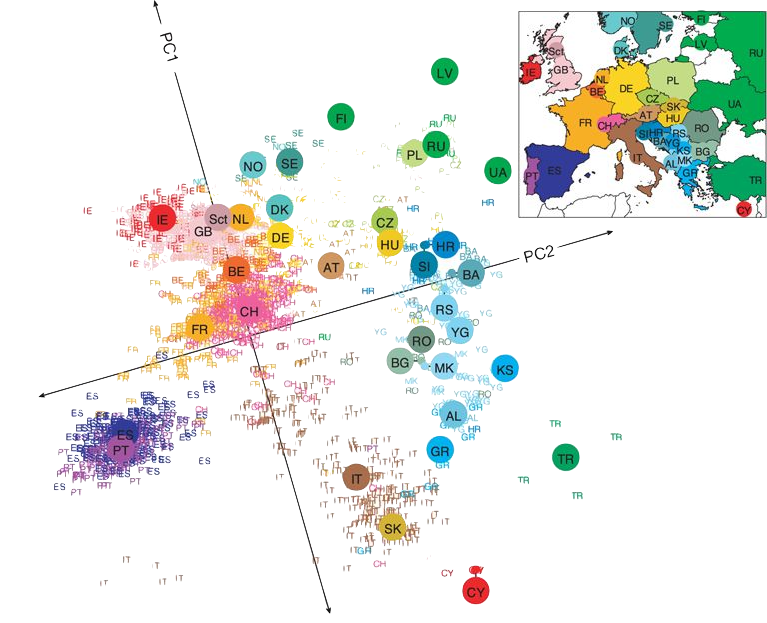
\includegraphics[width=.65\textwidth]{genes_pca.png}
	\end{center}
	\vspace{-.5em}
	\small
	Each data vector $\bv{x}_i$ contains genetic information for one person in Europe. Set $k = 2$ and plot $(XV)_i$ for each $i$ on a 2-d plane. Color points by what country they are from.  
\end{frame}



\begin{frame}
	\frametitle{semantic embeddings: motivating problem}
	Consider data sets which consist of text:
	
	\textbf{Review 1:} \textit{So far this thing is great. It takes up way less space and does a great job opening cans.}
	
	\textbf{Review 2:} \textit{Well designed, compact, and easy to use. I’ll never use another can opener.} 
	
	\textbf{Review 3:} \textit{Not entirely sure this was worth $20$. Mom couldn't figure out how to use it and it's fairly difficult to turn for someone with arthritis.}
	
	\begin{center}
		\textbf{\alert{Goal is to classify reviews as ``positive'' or ``negative''.}}
	\end{center}\end{frame}

\begin{frame}
	\frametitle{semantic embeddings: motivating problem}
	\textbf{Step 1:} Need to convert reviews to numerical data.
	
	\textbf{One approach:} Bag-of-words features.  
	
\end{frame}

\begin{frame}
		\frametitle{semantic embeddings: motivating problem}
		\small
		\textbf{Vocabulary:} Small, handy, excellent, great, quality, compact, easy, difficult.
		
		\textbf{Review 1:} \textit{Very small and handy for traveling or camping. Excellent quality, operation, and appearance..}
		
		\begin{align*}
		\left[\hspace{2em},\hspace{2em},\hspace{2em},\hspace{2em},\hspace{2em},\hspace{2em},\hspace{2em},\hspace{2em}\right]
		\end{align*}
		
		\textbf{Review 2:} \textit{So far this thing is great. Well designed, compact, and easy to use. I’ll never use another can opener.} 
		\begin{align*}
		\left[\hspace{2em},\hspace{2em},\hspace{2em},\hspace{2em},\hspace{2em},\hspace{2em},\hspace{2em},\hspace{2em}\right]
		\end{align*}
		
		\textbf{Review 3:} \textit{Not entirely sure this was worth $20$. Mom couldn't figure out how to use it and it's fairly difficult to turn for someone with arthritis.}
				\begin{align*}
		\left[\hspace{2em},\hspace{2em},\hspace{2em},\hspace{2em},\hspace{2em},\hspace{2em},\hspace{2em},\hspace{2em}\right]
		\end{align*}
\end{frame}

\begin{frame}
	\frametitle{semantic embeddings}
	\small
	\begin{center}
		This approach only works well for very large data sets. 
	\end{center}
	The algorithm is ignorant to a the fact that ``great'' and ``excellent'' are near synonyms. Or that ``difficult'' and ``easy'' are antonyms.
	
	\textbf{Goal:} Map words to numerical vectors in a \emph{semantically} meaningful way. Similar words map to similar vectors. Dissimilar words to dissimilar vectors.
	
	\begin{center}
		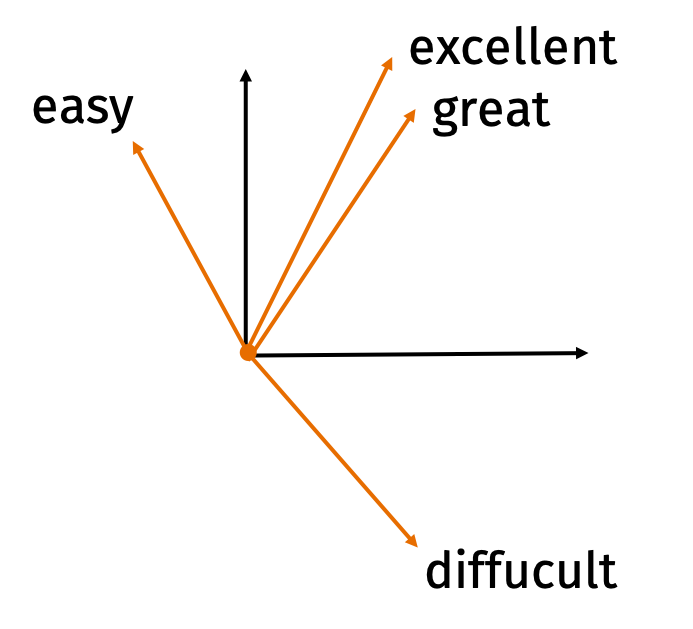
\includegraphics[width=.3\textwidth]{semantic_embedding.png}
	\end{center}
	
	
\end{frame}

\begin{frame}
	
	
\end{frame}

\begin{frame}
	\frametitle{latent semantic analysis}
	\begin{center}
		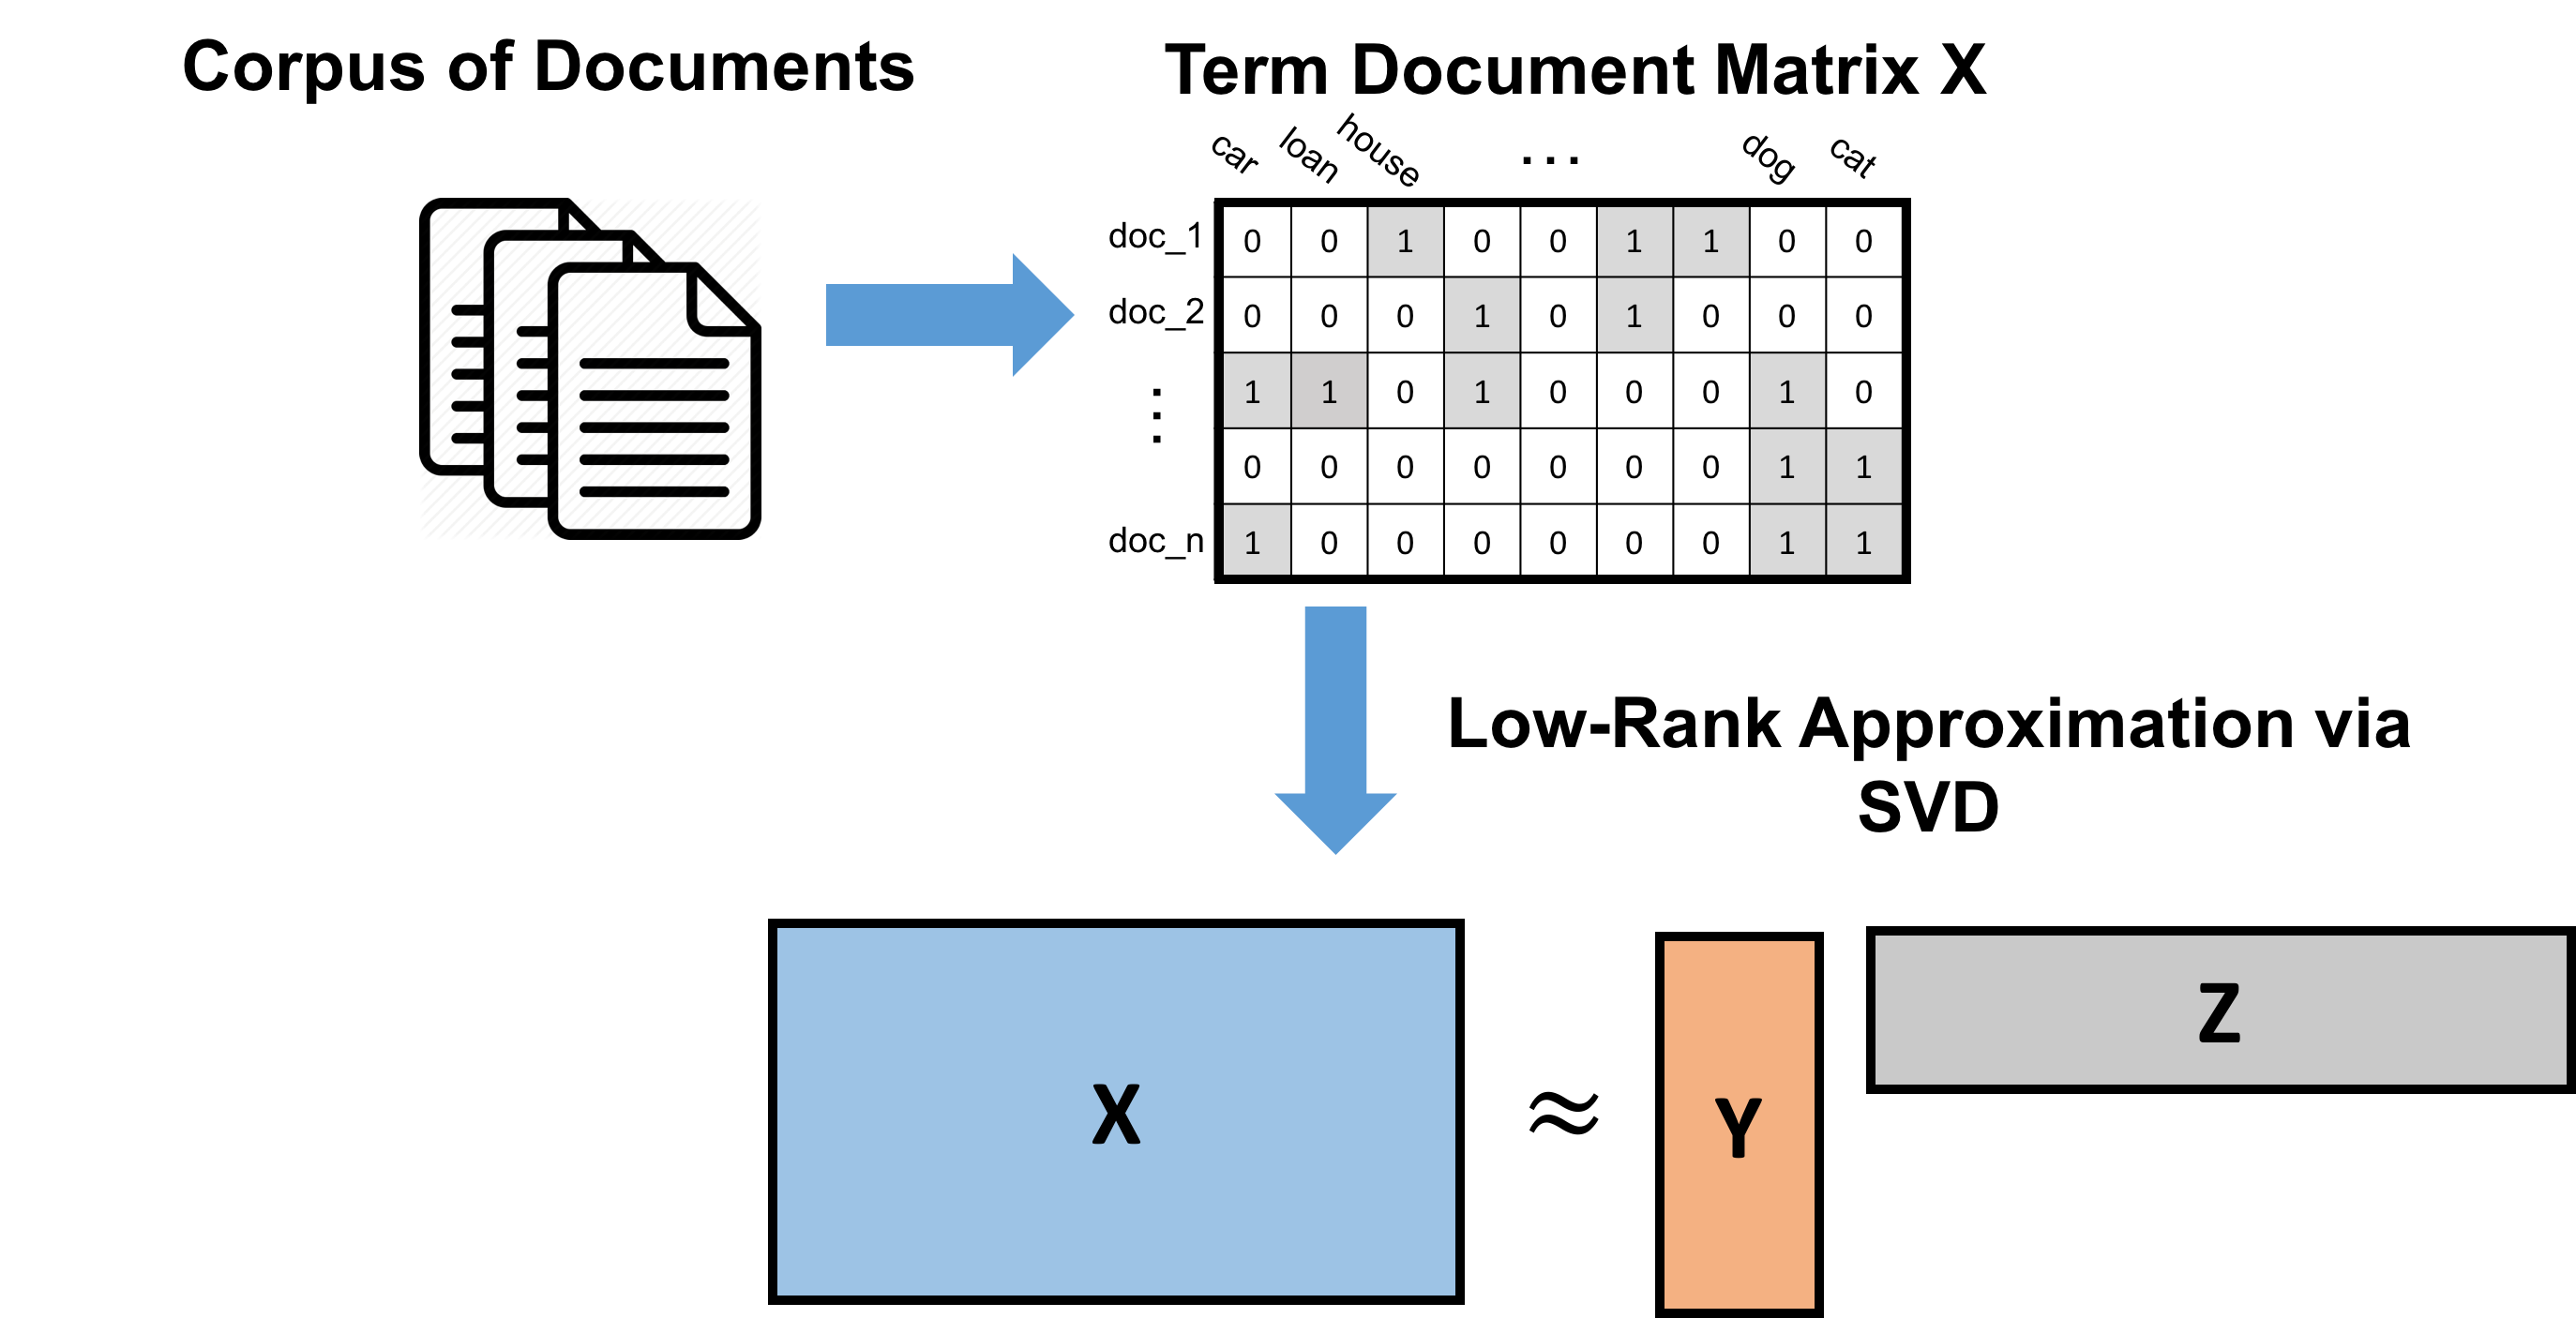
\includegraphics[width=.8\textwidth]{lsa.png}
	\end{center}
	\begin{itemize}
		\item $\langle \vec y_i, \vec z_a \rangle \approx 1$ when $doc_i$ contains $word_a$. 
		\item If $doc_i$ and $doc_i$ both contain $word_a$, $\langle \vec y_i, \vec z_a \rangle \approx \langle \vec y_j, \vec z_a \rangle = 1$.
	\end{itemize}
	\vspace{-2em}
	\begin{center}
		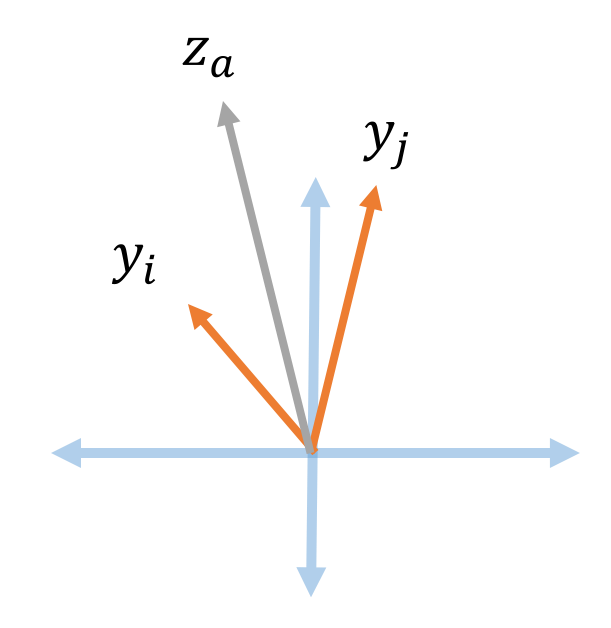
\includegraphics[width=.25\textwidth]{lsa2.png}
	\end{center}
\end{frame}

\begin{frame}
	\frametitle{example: latent semantic analysis}
	\begin{center}
		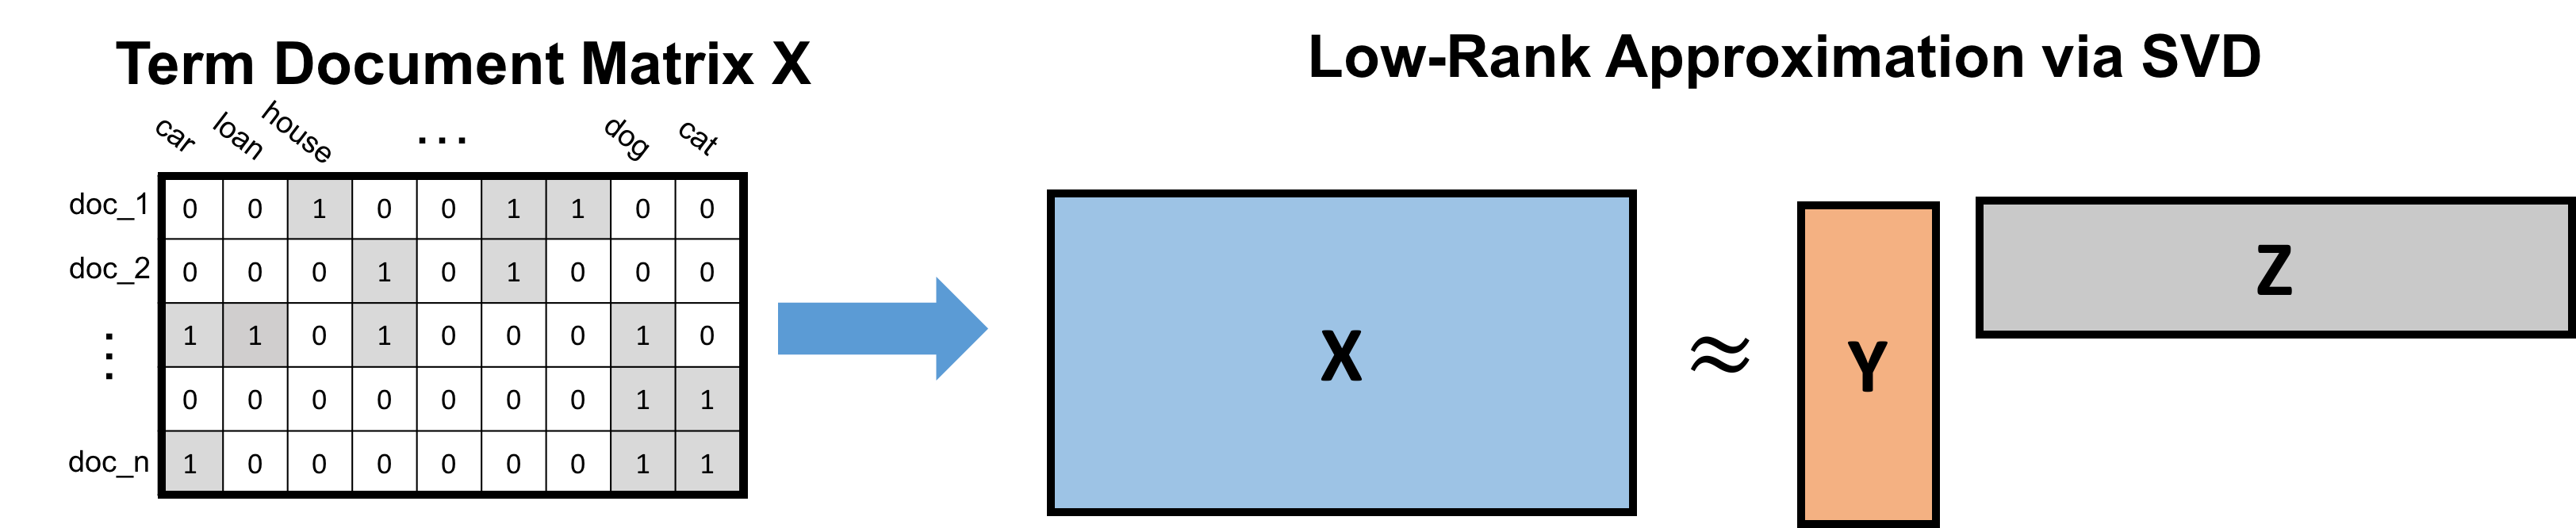
\includegraphics[width=.9\textwidth]{lsa3.png}
	\end{center}
	\vspace{-1em}
	\begin{itemize}
		\item The columns $\vec z_1, \vec z_2,\ldots $ give representations of words, with $\vec z_i$ and $\vec z_j$ tending to have high dot product if $word_i$ and $word_j$ appear in many of the same documents.
		\item  $\bv{Z}$ corresponds to the top $k$ right singular vectors: the eigenvectors of $\bv{X} \bv{X}^T$. \alert{Intuitively, what is $\bv{X} \bv{X}^T$?}
		\item $(\bv{X} \bv{X}^T)_{i,j} = $ 
	\end{itemize}
\end{frame}

\begin{frame}
	\frametitle{example: word embedding}
	Not obvious how to convert a word into a feature vector that captures the meaning of that word. Approach suggested by LSA: build a $d\times d$ symmetric ``similarity matrix'' $\bv{M}$ between words, and factorize: $\bv{M} \approx \bv{FF}^T$ for rank $k$ $\bv{F}$. 
	\vspace{5em}
	\begin{itemize}
		\item \textbf{Similarity measures:} How often do $word_i,word_j$ appear in the same sentence, in the same window of $w$ words, in similar positions of documents in different languages?
		\item Replacing $\bv{XX}^T$ with these different metrics (sometimes appropriately transformed) leads to popular word embedding algorithms: \texttt{word2vec}, \texttt{GloVe}, etc.
	\end{itemize}
\end{frame}

\begin{frame}
	\frametitle{example: word embedding}
	\begin{center}
		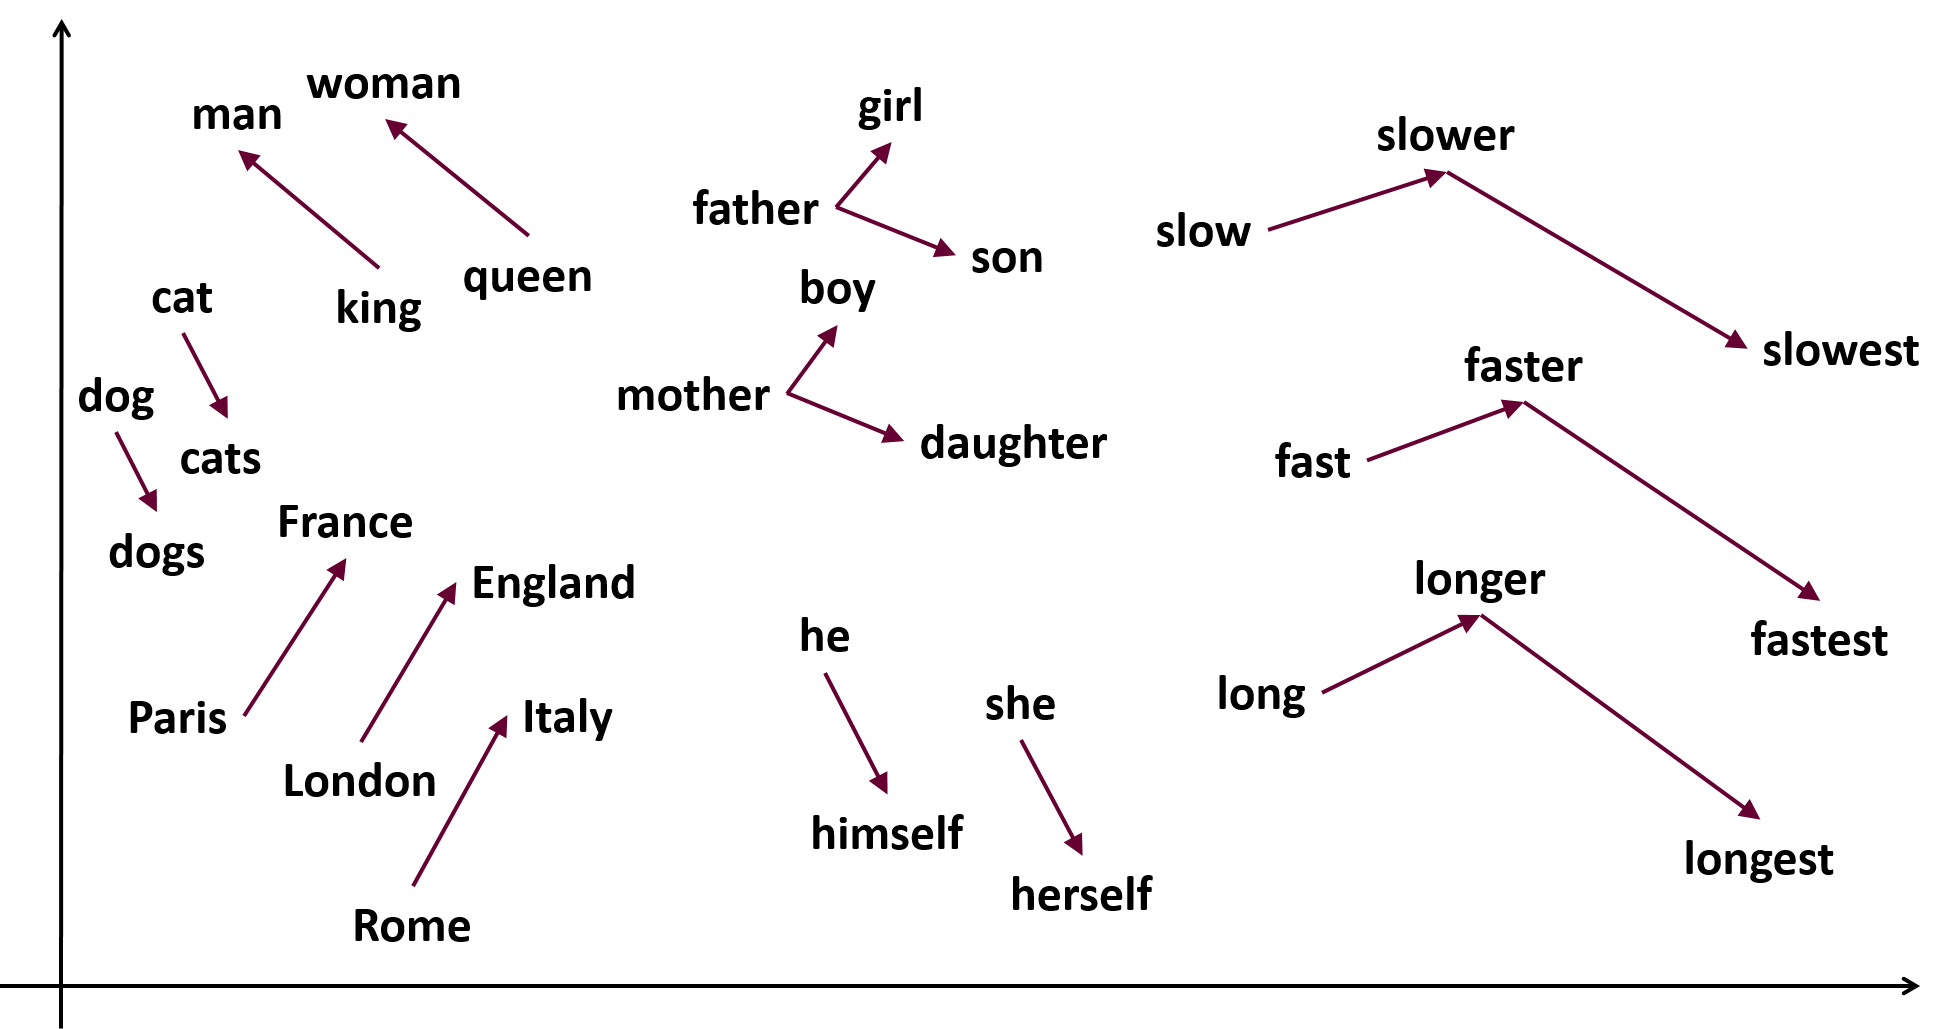
\includegraphics[width=.8\textwidth]{word2vec.png}
	\end{center}
	\begin{center}
		\texttt{word2vec} was originally described as a neural-network method, but Levy and Goldberg show that it is simply low-rank approximation of a specific similarity matrix. \textit{Neural word embedding as implicit matrix factorization.}
	\end{center}
\end{frame}


\end{document} 



